\documentclass[8pt]{beamer}

%%pacotes referentes ao Beamer
%\useoutertheme{split}
%\setbeamertemplate{navigation symbols}{}

%\usetheme{beamertheme}
%\usebeamercolor{beamer-color name}

%\usetheme{Boadilla}
%\usecolortheme{dove}

\usetheme{CambridgeUS}
\usecolortheme{beaver}

% \usetheme{pittsburgh}
% \usecolortheme{dolphin}
%\usecolortheme{dove}
%\usecolortheme{seahorse}

%\usetheme{Montpellier}

%number in figures an tables -- beamer
\setbeamertemplate{caption}[numbered]

%Colocar no description
%[leftmargin=!,labelwidth=\widthof{Turma A}]
	
%pacotes usuais do latex
\usepackage[portuguese]{babel}
\usepackage[utf8]{inputenc}
\usepackage{bm}
\usepackage{graphicx}
\usepackage{subfigure}
\usepackage[round]{natbib}
\usepackage{tikz}
\usetikzlibrary{shapes,arrows}
\usepackage{natbib}
\usepackage{times}
\usepackage{calc} %computes the length of a string
\usepackage{dsfont} %pacote para o 1 estilisado para indicadora
\usepackage{enumerate} %permite fazer uns enumerates diferentes
\usepackage[font=small,labelfont=bf]{caption} %permite colocar um segundo caption
\usepackage{booktabs} % comando \toprule, \midrule e \bottomrule
\usepackage{times} %times new roman font
\usepackage{multirow} %comando \multirow
\usepackage{setspace}
\usepackage{xcolor} %texto colorido
\usepackage{booktabs} %costumized tabs
%\usepackage{physics} %absolute value


%código para alinhar a esquerda os itens no description
\defbeamertemplate{description item}{align left}{\insertdescriptionitem\hfill}
\defbeamertemplate{enumerate item}{align left}{\insertdescriptionitem\hfill}



%AMS packages
\usepackage{amsmath}
\usepackage{amsfonts}
\usepackage{amssymb}

%Não quebre linhas
\binoppenalty=\maxdimen
\relpenalty=\maxdimen

%Comandos criados por mim
\DeclareMathOperator*{\argmin}{arg\,min}

\DeclareMathOperator*{\argmax}{arg\,max}


\DeclareMathOperator{\espe}{E}

\DeclareMathOperator{\spann}{span}

\DeclareMathOperator{\cov}{Cov}

\DeclareMathOperator{\vari}{Var}

%Informações para o primeiro slide
\date{}
\title[Estimação]{Estimação pontual e intervalo de confiança}
\author[Gilberto Sassi]{Gilberto Pereira Sassi}
\institute[IME -- UFBA]{Universidade Federal da Bahia \\ Instituto de Matem\'{a}tica e Estat\'{i}stica\\ Departamento de Estat\'{i}stica }

\begin{document}
	
\tikzstyle{decision} = [diamond, draw, fill=blue!20, 
text width=4.5em, text badly centered, node distance=3cm, inner sep=0pt]
\tikzstyle{block} = [rectangle, draw, fill=blue!20, 
text width=5em, text centered, rounded corners, minimum height=4em]
\tikzstyle{line} = [draw, -latex]
\tikzstyle{cloud} = [draw, ellipse,fill=red!20, node distance=3cm,
minimum height=2em]
	
\begin{frame}{}
	\maketitle
\end{frame}

\section{Estimação pontual}

\begin{frame}{}

% {\tiny
%  \begin{block}{Estimação pontual}
%   Encontrar o valor do parâmetro dos modelos de probabilidade.
%   
%    Seja $x_1, \dots, x_m$ os valores observados de uma variável quantitativa $X$ em uma amostra, então
%  \end{block}
%  
% 
% }

 {\tiny
 \begin{table}[ht]
  \centering
  \caption{Encontrar o valor do parâmetro dos modelos de probabilidade. \\ 
   Seja $x_1, \dots, x_m$ os valores observados de uma variável quantitativa $X$ em uma amostra, então:}
  \begin{tabular}{l|c|c|c}
  \toprule[0.05cm]
   Amostra & Distribuição & Parâmetros & Estimador\\
   \midrule[0.05cm]
   $X_1, \dots, X_m$ & $U_D[j, k]$ & $j$ & $\hat{j}=\min\{x_1, x_2, \dots, x_m\}$\\
   & $f(x) = \dfrac{1}{k-j+1},\quad x = j, \dots, k$ & $k$ & $\hat{k} = \max\{x_1, x_2, \dots, x_m\}$ \\ \midrule
   $X_1, \dots, X_m$ & $b(n, p)$ & $p$ & $\hat{p} = \dfrac{\bar{x}}{n} =  \dfrac{x_1+x_2 + \cdots + x_m}{n\cdot m}$\\
   & $f(x) = {n \choose x} p^x \cdot (1-p)^{n-x}, \quad x = 0, 1, \dots, n$ & $n$ conhecido &\\ \midrule
   $X_1, \dots, X_m$ & $Bernoulli (p)$ & $p$ & $\hat{p} = \bar{x} = \dfrac{x_1+x_2 + \cdots + x_m}{m}$\\
   & $f(x) = p^x \cdot (1-p)^{1-x},\quad x= 0, 1$ & &\\ \midrule
   $X_1, \dots, X_m$ & $Poison(\lambda)$ & $\lambda$ & $\hat{\lambda} = \bar{x} = \dfrac{x_1+x_2+\cdots+x_m}{m}$\\
   & $f(x) = \dfrac{e^{-\lambda}\lambda^x}{x!},\quad x=0,1,2,3,\cdots$ & & \\ \midrule
   $X_1, \dots, X_m$ & $U[a, b]$ & $a$ & $\hat{a}=\min\{x_1, x_2, \dots, x_m\}$\\
   & $f(x) = \dfrac{1}{b-a}, \quad x \in [a, b]$ & $b$ & $\hat{b}=\max\{x_1, x_2, \dots, x_m\}$ \\ \midrule
   $X_1, \dots, X_m$ & $Exponencial(\alpha)$ & $\alpha$ & $\hat{\alpha} = \dfrac{1}{\bar{x}}=  \dfrac{m}{x_1+x_2+\cdots+x_m} $\\
   & $f(x) = \alpha \exp(-\alpha x),\quad x \geq 0$ && \\ \midrule
   $X_1, \dots, X_m$ & $Normal(\mu, \sigma^2)$ & $\mu, \sigma^2$ & $\hat{\mu} =  \dfrac{x_1+x_2 + \cdots + x_m}{m}$\\
   & $f(x) = \dfrac{1}{\sqrt{2\pi \sigma^2}} \exp\left( -\dfrac{(x-\mu)^2}{2\sigma^2} \right)$ && $\hat{\sigma}^2 = \dfrac{(x_1-\hat{\mu})^2+(x_2-\hat{\mu})^2+ \cdots +
   (x_m-\hat{\mu})^2}{m-1} $ \\ 
   \bottomrule[0.05cm]
  \end{tabular}
 \end{table}
 }
 
\end{frame}

\begin{frame}{Exemplo -- Bernoulli}
 Um pesquisador está interessado em estudar a prevalência de um certa patologia. Para isso, ele coletou uma amostra em três etapas:
 \begin{enumerate}
  \item Na primeira etapa, ele coletou 5 pacientes e dois estavam infectados;
  \item Na segunda etapa, ele coletou 8 pacientes e 4 estavam infectados;
  \item Na terceira etapa, ele coletou 10 pacientes e 3 estavam infectados.
 \end{enumerate}
 Qual a prevalência desta patologia na população?
 \vfill
 
 \textbf{Solução:} Nesse caso, temos que 
 \begin{itemize}
  \item Sucesso: o paciente estar infectado;
  \item Probabilidade de sucesso: é a prevalência e precisamos estimar.
 \end{itemize}
Neste caso, temos uma variável aleatória com Distribuição Bernoulli. O tamanho final da amostra é $n=5+8+10=23$ e número de sucessos foi $2+4+3=9$, então a prevalência é aproximada por
\begin{align*}
 \hat{p} = \dfrac{9}{23}=0,39.
\end{align*}
\end{frame}

\begin{frame}{Exemplo -- Exponencial}

{\scriptsize
 Um profissional de saúde acompanhou 15 pacientes com certa patologia em estado avançado e observou o tempo em dias até o óbito obtendo os valores da tabela \ref{tab:exe_exp}.
 \begin{table}[ht]
\centering
\begin{tabular}{c|cccccccccc}
  \toprule[0.05cm]
Tempo até o óbito & 80 & 327 & 95 & 146 & 3 & 82 & 4 & 1152 & 226 & 173 \\ 
   \bottomrule[0.05cm]
\end{tabular}
\caption{Tempo (em dias) até óbito.} 
\label{tab:exe_exp}
\end{table}
Qual o modelo de probabilidade adequado neste contexto? Qual o parâmetro da distribuição que você escolheu? Qual um paciente em estado crítico com esta patologia viver mais de 180
dias?
\vfill

\textbf{Solução:} O tempo até um evento (o óbito nesse caso) é modelado usando a distribuição exponencial. O tempo médio até o óbito é 
\begin{align*}
 \bar{x} = \dfrac{80 + 327 + 95 + 146 + 3 + 82 + 4 + 1152 + 226 + 173}{10} = 228,8,
\end{align*}
e a taxa do modelo exponencial é aproximada por $\hat{\alpha} = \dfrac{1}{\bar{x}} = \dfrac{1}{228,8} = 0,004$.

A probabilidade de um paciente em estado crítico sobreviver mais de 180 dias é 
\begin{align*}
 P(X \geq 180) &= 1 - P(X < 180) \\
 &= 1 -\Big(1- \exp(-0.004\cdot 180)\Big)\\
 &= \exp(-0,004\cdot 180)\\
 &= 0,49.
\end{align*}
}
\end{frame}



% \section{Distribuição amostral}
% 
% \begin{frame}{Exemplo de motivação}
% 
% {\scriptsize
% Imagine que um professor tem uma turma com 30 alunos. As notas finais destes 30 alunos estão na Tabela~\ref{tab:dist_amostral}. Este professor está com tempo limitado e decidiu analisar o desempenho de 5 alunos ao final do curso. Existem $142.506$ maneiras de selecionar esses cinco alunos. Na Tabela~\ref{tab:amostras}, mostramos dez amostras diferentes com cinco alunos. Note que cada amostra tem uma média diferente. \textcolor{blue}{A ideia é que a média é uma variável (valor diferente em cada amostra) que denotamos por $\bar{X}$}.
% 
% 
% \begin{table}[ht]
% 	\centering
% 	\begin{tabular}{cccccccccc}
% 		\toprule[0.05cm]
% 		7,29 & 7,19 & 7,15 & 5,54 & 5,93 & 5,53 & 6,44 & 6,27 & 8,16 & 5,72 \\ 
% 		4,84 & 4,63 & 6,11 & 7,10 & 3,37 & 7,36 & 6,70 & 5,70 & 6,31 & 7,64 \\ 
% 		5,89 & 8,82 & 7,77 & 7,93 & 5,24 & 6,08 & 5,77 & 6,57 & 6,00 & 6,14 \\ 
% 		\bottomrule[0.05cm]
% 	\end{tabular}
% 	\caption{Turma com 30 alunos.} 
% 	\label{tab:dist_amostral}
% \end{table}
% 
% 
% 
% \begin{table}[ht]
% 	\centering
% 	\begin{tabular}{l|ccccc|c}
% 		\toprule[0.05cm]
% 		Amostras & Aluno 1 & Aluno 2 & Aluno 3 & Aluno 4 & Aluno 5 & Média da amostra \\ 
% 		\midrule[0.05cm]
% 		Amostra 1 &7,19 & 8,82 & 5,54 & 6,70 & 6,11 & 6,87 \\ 
% 		Amostra 2 &7,36 & 4,84 & 6,31 & 6,27 & 7,29 & 6,41 \\ 
% 		Amostra 3 & 5,77 & 6,57 & 6,44 & 8,16 & 7,93 & 6,97 \\ 
% 		Amostra 4 & 6,44 & 7,29 & 5,77 & 3,37 & 6,11 & 5,80 \\ 
% 		Amostra 5 & 6,14 & 7,36 & 3,37 & 6,70 & 7,10 & 6,13 \\ 
% 		Amostra 6 & 8,82 & 6,31 & 7,36 & 5,77 & 5,72 & 6,80 \\ 
% 		Amostra 7 & 7,10 & 7,93 & 4,84 & 6,44 & 5,93 & 6,45 \\ 
% 		Amostra 8 & 7,10 & 5,72 & 7,36 & 5,77 & 4,84 & 6,16 \\ 
% 		Amostra 9 & 6,44 & 6,14 & 7,64 & 6,08 & 5,70 & 6,40 \\ 
% 		Amostra 10 & 6,00 & 7,77 & 5,53 & 5,24 & 7,15 & 6,34 \\ 
% 		\bottomrule[0.05cm]
% 	\end{tabular}
% 	\caption{Dez amostras com cinco alunos com a média.} 
% 	\label{tab:amostras}
% \end{table}
% }
% \end{frame}
% 
% %\begin{frame}{Introdução}
% %\begin{block}{Objetivo}
% % A ideia é que podemos a média (calculada em diversas amostras) é uma variável que denotamos por $\bar{X}$. Podemos calcular medidas de resumo para $\bar{X}$ e construir um histograma para $\bar{X}$, por exemplo. Além disso, $\bar{X}$ encontrar um modelo de probabilidade adequado para $\bar{X}$.
% %\end{block}
% %
% %\begin{block}{Exemplo de motivação}
% % Um jogo consiste em lançar uma moeda honesta 3 vezes. Para cada lançamento, se sair cara você ganha um ponto, caso saia coroa, você perde um ponto. Podemos construir uma variável aleatória discreta:
% % \begin{align*}
% %  X = \begin{cases}
% %       1, & \mbox{ se sair cara},\\
% %       -1, & \mbox{ se sair coroa},
% %      \end{cases}
% % \end{align*}
% % com função de probabilidade $f(1) = 0,5 = f(-1)$. Então podemos ter as seguintes amostras:
% %\end{block}
% %
% % 
% %\end{frame} 
% 
% %\begin{frame}{Exemplo de motivação}
% %
% %  {\small
% %  \begin{table}[ht]
% %   \centering
% %   \caption{}
% %   \begin{tabular}{l|c|c}
% %    \toprule[0.05cm]
% %    $X_1, X_2, X_3$ & Probabilidade & $\bar{X} = \dfrac{X_1+X_2+X_3}{3}$ \\ 
% %    \midrule[0.05cm]
% %    $-1,-1,-1,$ & $\frac{1}{8}$ & $-1$ \\ \hline
% %    $-1,-1,1$ & $\frac{1}{8}$  & $-\frac{1}{3}$\\ \hline
% %    $-1, 1, -1$ & $\frac{1}{8}$  & $-\frac{1}{3}$\\ \hline
% %    $-1, 1, 1$ & $\frac{1}{8}$ & $\frac{1}{3}$ \\ \hline
% %    $1, -1, -1$ & $\frac{1}{8}$ & $-\frac{1}{3}$\\ \hline
% %    $1, -1, 1$ & $\frac{1}{8}$ & $\frac{1}{3}$ \\ \hline
% %    $1,1,-1$ & $\frac{1}{8}$ & $\frac{1}{3}$ \\ \hline
% %    $1,1,1$ & $\frac{1}{8}$ & 1 \\ \bottomrule[0.05cm]
% %   \end{tabular}
% %  \end{table}
% %  }
% %
% %\end{frame}
% 
% %\begin{frame}{Exemplo de motivação}
% % Assim, notamos que $\bar{X}$ é uma variável com valores possíveis $-1, \frac{-1}{3}$, $\frac{1}{3}, 1$ e função de probabilidade
% % \begin{table}[ht]
% %  \centering
% %  \caption{}
% %  \begin{tabular}{l|cccc}
% %  $\bar{X}$ & $-1$ & $-\frac{1}{3}$ & $\frac{1}{3}$ & $1$\\ \midrule[0.05cm]
% %  $p$ & $\frac{1}{8}$ & $\frac{3}{8}$ & $\frac{3}{8}$ & $\frac{1}{8}$ \\
% %  \end{tabular}
% % \end{table}
% %
% %  Note que neste exemplo conseguimos enumerar os valores possíveis de $\bar{X}$, mas isso nem sempre é possível ou fácil. 
% %  
% %  \begin{block}{Propriedade IMPORTANTE da distribuição Normal}
% %  \textcolor{red}{Se $x_1, \dots, x_m$ valores observados da variável aleatória $X \sim N(\mu, \sigma^2)$, então  $\bar{X} \sim Normal\left( \mu, \frac{\sigma^2}{n} \right)$.}
% %  \end{block}
% %
% %  
% %\end{frame}
% 
% %\begin{frame}{Exemplo}
% % Em um estudo da altura de pacientes, escolhemos 10 pacientes. Sabemos que a altura dos pacientes tem distribuição normal com média $185cm$ e desvio padrão $40cm$. Qual a distribuição de $\bar{X}$?
% % Qual a probabilidade da altura média dos pacientes escolhidos ser maior que a média populacional?
% % \vfill
% % 
% % \textbf{Solução:}
% % 
% % \begin{itemize}
% %  \item $\bar{X} \sim Normal\left( 185, \dfrac{40}{10}  \right) $, ou seja, $\bar{X} \sim Normal\left( 185, 4 \right)$.
% %  \vfill
% %  
% %  \item
% %  \begin{align*}
% %   P(\bar{X} > 185) &= 1 - P(\bar{X} \leq 185)\\
% %   &= 1 - \Phi\left( \dfrac{\bar{X}-185}{2} \right)\\
% %   &= 1 - \Phi(0) = 1 - 0,50 = 0,50
% %  \end{align*}
% % \end{itemize}
% %
% % 
% %\end{frame}
% 
% \section{Teorema central do limite}
% 
% \begin{frame}{Teorema central do limite}
% \begin{block}{Ideia}
%  Para um tamanho de amostra suficientemente grande, a distribuição de $\bar{X}$ pode ser aproximada por uma distribuição normal, independente do modelo de probabilidade de $X_i$.
% \end{block}
% \vfill
% 
% \begin{block}{Teorema central do limite (amostras grandes)}
%  Considere uma população com média $\mu$ e $\sigma^2$. Suponha que temos uma amostra $X_1, \dots, X_n$, então
%  \begin{align*}
%   \bar{X}  \sim Normal\left(\mu, \dfrac{\sigma^2}{n} \right).
%  \end{align*}
% \end{block}
% \vfill
% 
% \begin{block}{Propriedade IMPORTANTE da distribuição Normal}
% 	\textcolor{red}{Se $x_1, \dots, x_m$ valores observados da variável aleatória $X \sim N(\mu, \sigma^2)$, então  $\bar{X} \sim Normal\left( \mu, \frac{\sigma^2}{n} \right)$.}
% \end{block}
% \end{frame}
% 
% \begin{frame}{Exemplo}
% Em um estudo da altura de pacientes, escolhemos 10 pacientes. Sabemos que a altura dos pacientes tem distribuição normal com média $185cm$ e desvio padrão $40cm$. Qual a distribuição de $\bar{X}$?
% Qual a probabilidade da altura média dos pacientes escolhidos ser maior que a média populacional?
% \vfill
% 
% \textbf{Solução:}
% 
% \begin{itemize}
% 	\item $\bar{X} \sim Normal\left( 185, \dfrac{40}{10}  \right) $, ou seja, $\bar{X} \sim Normal\left( 185, 4 \right)$.
% 	\vfill
% 	
% 	\item
% 	\begin{align*}
% 	P(\bar{X} > 185) &= 1 - P(\bar{X} \leq 185)\\
% 	&= 1 - \Phi\left( \dfrac{185-185}{2} \right)\\
% 	&= 1 - \Phi(0) = 1 - 0,50 = 0,50
% 	\end{align*}
% \end{itemize}
% 
% 
% \end{frame}
% 
% 
% \begin{frame}{Exemplo}
% Considere uma variável aleatória discreta $X: \Omega \rightarrow \mathbb{R}$ que assume os valores $3, 6$, e $8$ com, respectivamente, probabilidades $0,5; 0,3$, e $0,2$. Uma amostra de 40 observações é 
% sorteada, qual a probabilidade da média da amostra ser maior que 5?
% \vfill
% 
% \textbf{Solução:} Primeiramente, note que
% \begin{align*}
%  \mu &= 0,4 \cdot 3 + 0,3 \cdot 6 + 0,2 \cdot 8 = 4,9,\\
%  \sigma^2 &= 0,4 \cdot (3 - 4,9)^2 + 0,3 \cdot (6 - 4,9)^2 + 0,3 \cdot (8 - 4,9)^2 = 4,09.
% \end{align*}
% 
% Usando o Teorema central do limite, temos que $\bar{X} \sim N\left(4,9; \dfrac{4,09}{40}\right)$ e 
% \begin{align*}
%  P(\bar{X} > 5) &=1-  P(\bar{X} \leq 5)\\
%  &=1- \Phi \left( \dfrac{5 - 4,9}{\sqrt{ \frac{4,09}{40} }} \right)\\
%  &= 1 - \Phi(0,32) = 1-0,6255=0,37.
% \end{align*}
% 
%  
% \end{frame}
% 
% 
% \subsection{Distribuição Bernoulli}
% 
% \begin{frame}{Exemplo}
% \begin{block}{Distribuição Bernoulli}
%  Lembre que $\espe (X) = p$ e $\vari(X) = p(1-p)$.
% \end{block}
% 
% \begin{block}{Exemplo}
%  Suponha que a prevalência do vírus HIV na África Subsariana é $10\%$. Um médico selecionou 40 pacientes desta região. Qual a probabilidade de no máximo $20\%$ desses pacientes estarem infectados pelo vírus?
%  \vfill
%  
%  \textbf{Solução:}  Pelo Teorema central do limite, temos que $\hat{p}  \sim N\left(0,1; \dfrac{0,1\cdot 0,9}{40}\right)$. Logo, temos que
%  \begin{align*}
%   P(\hat{p} < 0,2) &= \Phi \left(\dfrac{0,2 - 0,1}{ \sqrt{ \frac{0,1 \cdot 0,9}{40} } }\right) \\
%   &= \Phi( 2,11)=0,9826
%  \end{align*}
% 
% \end{block}
% 
%  
% \end{frame}
% 
% \subsection{Distribuição poison}
% 
% \begin{frame}{Exemplo}
% 
% \begin{block}{Distribuição poison}
% Lembre que $\espe(X) = \lambda$ e $\vari(X) = \lambda$.
% \end{block}
% 
% 
% \begin{block}{Exemplo}
%  A emissão de partículas radioativas alfa de um isótopo em um minuto é modelada através de um distribuição poison com média 5. 
%  Um físico analisar cinco amostras desse isótopo e observou o número de partículas alfa emitidas para  uma amostra com observações $x_1, x_2, x_3, x_4, x_5$. 
%  Qual a probabilidade da média de partículas emitidas nessa amostra com cinco valores ser maior que seis?
%  \vfill
%  
%  \textbf{Solução:} Pelo teorema central do limite, temos que $\bar{X} \sim N\left(\lambda, \dfrac{\lambda}{5}\right)$. Então
%  
%  \begin{align*}
%   P(\bar{X} > 6) &= 1 - P(\bar{X} \leq 6)\\
%   &= 1 - \Phi\left( \dfrac{6-5}{\sqrt{ \frac{5}{5} }} \right)\\
%   &= 1 - \Phi( 1) = 1 - 0,8413 = 0,1587
%  \end{align*}
% 
% \end{block}
% \end{frame}
% 
% \subsection{Distribuição exponencial}
% 
% \begin{frame}{Exemplo}
%  \begin{block}{Distribuição exponencial}
%  Lembre que $\espe(X) = \frac{1}{\alpha}$ e $\vari(X) = \frac{1}{\alpha^2}$.
%  \end{block}
% 
%  \begin{block}{Exemplo}
%  Uma indústria fabrica lâmpadas especiais que ficam em operação continuamente. A fabricante afirma que as lâmpadas duram em média 8000 horas. 
%  Um órgão de controle teste 10 lâmpadas. Assumindo que o fabricante diz a verdade, qual a probabilidade do órgão regulador obter uma média de no máximo 7000 horas para a amostra?
%  \vfill
%  
%  \textbf{Solução:} Pelo teorema do limite central, temos que $\bar{X} \sim N\left( \dfrac{1}{\alpha}; \dfrac{1}{\alpha^2\cdot m} \right)$. Então,
%  \begin{align*}
%   P(\bar{X} < 7000) &= \Phi\left( \dfrac{7000 - \dfrac{1}{\alpha}}{\dfrac{1}{\alpha^2\cdot m}}  \right) = \Phi \left( \dfrac{7000 - \dfrac{1}{8000}}{\dfrac{1}{8000^2\cdot 10}} \right)\\
%   &= \Phi( -0,4) \\
%   &= 1 - \Phi(Z < 0,4) = 1- 0,6554 = 0.3446 \approx 0.34
%  \end{align*}
% 
%  \end{block}
% \end{frame}
% 



\section{Estimação intervalar -- população com distribuição normal e $\sigma^2$ conhecida}

\begin{frame}{Organização dos intervalos de confiança}
	
\huge 
	\begin{enumerate}
		\item Distribuição normal:
		\begin{enumerate}
			\item Intervalo de confiança para média quando variância é conhecida (intervalos $Z$);
			\item Intervalo de confiança para média quando variância é desconhecida (intervalos $t$);
			\item Intervalo de confiança para variância;
		\end{enumerate}
		\vfill
		
		\item Distribuição exponencial:
		\begin{enumerate}
			\item Intervalo de confiança para o tempo médio de vida ou duração;
		\end{enumerate}
		\vfill
		
		\item Grandes amostras (tamanho da amostra $\geq 40$):
		\begin{enumerate}
			\item Intervalo de confiança para proporção para distribuição Bernoulli;
			\item Intervalo de confiança  para outras distribuições.
		\end{enumerate}
	\end{enumerate}

\normalsize
\end{frame}

\small
\begin{frame}{Estimação intervalar para média $\mu$\\ Distribuição normal com $\sigma^2$ conhecida}
 \begin{block}{Objetivo}
  Agora queremos encontrar um intervalo de valores plausíveis para o parâmetro $\mu$, ou seja, queremos encontrar $a$ e $b$ tal que \textcolor{blue}{$a < \mu < b$} com uma medida de \textit{precaução ou prudência} $\gamma$, ou seja, se repetirmos o experimento ou a amostragem, $95\%$ das amostras produziriam um intervalo que contém o parâmetro.
  \vspace{0.25cm}
  
  Chamamos \textcolor{blue}{$(a, b)$} de intervalo de confiança e acreditamos que este intervalo está correto com uma medida de \textit{precaução ou prudência}   $ \gamma$. Chamamos $\gamma$ de coeficiente de confiança.
 \end{block}
\vfill

Suponha que você conhece o desvio padrão $\sigma$ populacional da variável aleatória contínua $X$ com distribuição normal. Seja $x_1, \dots, x_n$ uma amostra de tamanho $n$ da variável $X$, então o intervalo de confiança para a média populacional $\mu$ com coeficiente de confiança $\gamma = 1 - \alpha$ 
é dado por
\begin{align*}
IC(\mu; \gamma) = \left( -z_{1-\frac{\alpha}{2}}\dfrac{\sigma}{\sqrt{n}} + \bar{x}; z_{1-\frac{\alpha}{2}}\dfrac{\sigma}{\sqrt{n}} + \bar{x} \right)
\end{align*}
em que $\Phi(z_{1-\frac{\alpha}{2}}) = \frac{\gamma + 1}{2} = 1 - \frac{\alpha}{2}$. Algumas vezes, usamos a notação $\bar{x} \pm z_{1-\frac{\alpha}{2}} \frac{\sigma}{\sqrt{n}}$.
\end{frame}
\normalsize

\begin{frame}{Interpretação do coeficiente de confiança}

Gostaríamos de reforçar que o intervalo de confiança é um processo de generalização de uma amostra para toda população. Existe uma possibilidade dessa generalização estar errada como ilustrado na Tabela~\ref{fig:confianca}.

%\begin{figure}[htbp]
%	\caption{População com notas de 30 alunos e intervalos de confiança com coeficiente de confiança $\gamma=0,95$ para seis amostras de cinco alunos.}
%	\centering
%	\label{fig:confianca}
%	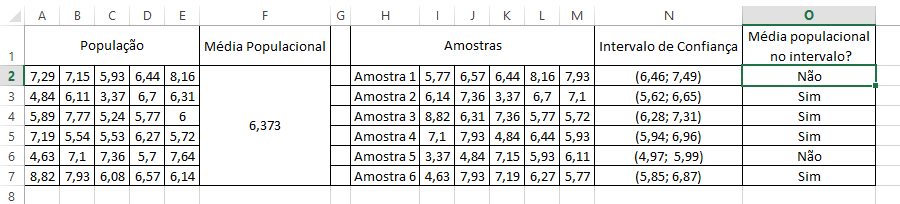
\includegraphics[width=12cm]{confianca.png}
%\end{figure}


\scriptsize
\begin{table}[htbp]
	\caption{Intervalos de confiança e amostras de uma população com distribuição normal com média populacional $\mu=1,75$ e desvio padrão $\sigma=0,1$.}
	\begin{tabular}{|c|c|r|r|r|r|r|r|r|c|}
		\hline
		\multicolumn{1}{|c|}{$\mu$} &  & \multicolumn{ 5}{c|}{Amostra} & \multicolumn{1}{c|}{a} & \multicolumn{1}{c|}{b} & $a < \mu < b$? \\ \hline
		\multirow{3}{*}{1,75} & Amostra 1 & 2,050 & 1,909 & 1,893 & 1,858 & 1,651 & 1,785 & 1,960 & Não \\ \cline{ 2- 10}
 & Amostra 2 & 1,667 & 1,909 & 1,958 & 1,771 & 2,028 & 1,779 & 1,954 & Nao \\ \cline{ 2- 10}
 & Amostra 3 & 1,835 & 1,905 & 1,995 & 1,805 & 1,820 & 1,784 & 1,960 & Não \\ \hline
		\multicolumn{1}{|c|}{$\sigma$} & Amostra 4 & 1,824 & 1,870 & 1,965 & 1,637 & 1,711 & 1,714 & 1,889 & Sim \\ \hline
		\multirow{2}{*}{0,1} & Amostra 5 & 1,773 & 1,796 & 1,895 & 1,872 & 1,812 & 1,742 & 1,917 & Sim \\ \cline{ 2- 10}
 & Amostra 6 & 1,741 & 1,885 & 1,896 & 1,629 & 1,664 & 1,675 & 1,851 & Sim \\ \hline
	\end{tabular}
	\label{fig:confianca}
\end{table}


\normalsize



Na Tabela~\ref{fig:confianca}, o intervalo de confiança com coeficiente de confiança $\gamma=0,95$ pode ou não conter a média populacional. \textcolor{blue}{ O importante é que $95\%$ dos intervalos de confiança vão conter a média populacional já que $\gamma = 0,95$}. Ou seja, de $100$ intervalos de confianças de distintas amostras, aproximadamente $95$ intervalos vão conter a média populacional. Ilustramos esta ideia na Figura~\ref{fig:interpretacao_confianca}.
 \end{frame}

\begin{frame}{Interpretação do coeficiente de confiança}
\begin{figure}[htbp]
	\centering
	\caption{Interpretação do coeficiente de confiança.}
	\label{fig:interpretacao_confianca}
	\begin{tikzpicture}[scale=0.6]
	\draw (0,-2) -- (0,7);
	\node[above] at (0,7)  {{\LARGE $\mu$}};
	\draw (-2,6) -- (2,6);
	\node[right] at (4,6) {{\large Amostra 1}};
	\draw (-2,6-0.1) -- (-2,6+0.1);
	\draw (2,6-0.1) -- (2,6+0.1);
	\draw (-1,5) -- (3,5);
	\node[right] at (4,5) {{\large Amostra 2}};
	\draw (-1,5-0.1) -- (-1,5+0.1);
	\draw (3,5-0.1) -- (3,5+0.1);
	\draw (-3,4) -- (1,4);
	\node[right] at (4,4) {{\large Amostra 3}};
	\draw (-3,4-0.1) -- (-3,4+0.1);
	\draw (1,4-0.1) -- (1,4+0.1);
	\draw (-5,3) -- (-1,3);
	\node[right] at (4,3) {{\large Amostra 4}};
	\draw (-5,3-0.1) -- (-5,3+0.1);
	\draw (-1,3-0.1) -- (-1,3+0.1);
	\node at (-1, 1) {{\LARGE $\vdots$}};
	\node at (1,1) {{\LARGE $\vdots$}};
	\draw (-1,-1) -- (3,-1);
	\node[right] at (4,-1) {{\large Amostra 100}};
	\draw (-1,-1-0.1) -- (-1,-1+0.1);
	\draw (3,-1-0.1) -- (3,-1+0.1);
	\end{tikzpicture}
\end{figure}

\end{frame}

\begin{frame}{Exemplo}

{\small
 Suponha que os comprimentos de jacarés de um certa raça tenham variância $\sigma^2=0,01m^2$. Uma amostra de dez animais foi coletada e forneceu uma média de $1,69m$. Construa um intervalo de confiança
 com coeficiente de confiança $\gamma = 0,95$. Construa um intervalo de confiança para a média da população de jacarés com coeficiente de confiança $\gamma = 99\%$.
 \vfill

 \textbf{Solução:}
 \begin{itemize}
  \item Para $\gamma = 95\%$. Primeiramente precisamos encontrar $z_{1-\frac{\alpha}{2}}$, ou seja,  $ \Phi(z_{1-\frac{\alpha}{2}}) = 1 - \frac{\alpha}{2} = 0,975 $. 
  
  Logo $z_{1-\frac{\alpha}{2}} = 1,96$. Então, o intervalo de confiança para a altura média do jacaré é 
 \begin{align*}
  IC(\mu,95\%) = \left( -1,96 \cdot \sqrt{\dfrac{0,01}{10}} + 1,69;1,96 \cdot \sqrt{\dfrac{0,01}{10}} + 1,69 \right) = (1,63;1,75).
 \end{align*}
 Ou seja, com coeficiente de confiança $95\%$, a altura média do jacaré está entre $1,63m$ e $1,75m$.

 \item Para $\gamma = 99\%$. Primeiramente precisamos encontrar $z_{1-\frac{\alpha}{2}}$, ou seja,  $ \Phi(z_{1-\frac{\alpha}{2}}) = \dfrac{1+\gamma}{2} = 0,995$ e  $z_{1-\frac{\alpha}{2}} = 2,58$. Então, o intervalo de confiança para a altura média do jacaré é 
 \begin{align*}
  IC(\mu,95\%) = \left( -2,58 \cdot \sqrt{\dfrac{0,01}{10}} + 1,69;2,58 \cdot \sqrt{\dfrac{0,01}{10}} + 1,69 \right) = (1,60;1,77).
 \end{align*}
 Ou seja, com coeficiente de confiança $99\%$, a altura média do jacaré está entre $1,60m$ e $1,77m$.
 \end{itemize}
}
\end{frame}

\subsection{Tamanho da amostra}



\begin{frame}{Escolha do tamanho da amostra}

\small

\begin{block}{Precisão da estimativa}
	Quando usamos $\bar{x} = \frac{x_1 \dots + x_n}{n}$ para aproximar $\mu$, o erro $E = \lvert \bar{x} - \mu \rvert$ é menor ou igual a $ \frac{z_{1-\frac{\alpha}{2}} \sigma}{\sqrt{n}}$ com coeficiente de confiança $\gamma = 100(1-\alpha)\%$.conforme  ilustrado na Figura~\ref{fig:intervalo_conf}.
	
	\begin{figure}
		\centering
		\caption{Erro quando usamos $\bar{x}$ para aproximar $\mu$}
		\label{fig:intervalo_conf}
		\begin{tikzpicture}
			\draw[->] (-4,0) -- (4,0);
			\filldraw[blue] (-2,0) circle (1.5pt);
			\node[below] at (-2, 0) {\tiny $l=\bar{x} - \frac{z_{1-\frac{\alpha}{2}} \sigma}{\sqrt{n}}$};
			\filldraw[blue] (-1, 0) circle (1.5pt);
			\node[below] at (-1,0) {\tiny $\mu$};
			\filldraw[blue] (0,0) circle (1.5pt);
			\node[below] at (0,0) {\tiny $\bar{x}$};
			\filldraw[blue] (2, 0) circle (1.5pt);
			\node[below] at (2,0) {\tiny $u=\bar{x} + \frac{z_{1-\frac{\alpha}{2}} \sigma}{\sqrt{n}}$};
			\draw[red] (-1, 0.2) -- (-1, 0.4);
			\draw[red] (0, 0.2) -- (0, 0.4);
			\draw[red] (-1, 0.3) -- (0, 0.3);
			\node[above, right, red] at (-1.2, 0.5) {\tiny $E = erro = \lvert \mu - \bar{x} \rvert$};
		\end{tikzpicture}
	\end{figure}
	Note que $\frac{z_{1-\frac{\alpha}{2}} \sigma}{\sqrt{n}}$ aumenta quando aumentamos $\gamma$ (ou diminuímos $\alpha$).  \textcolor{blue}{Dizemos que $\frac{z_{1-\frac{\alpha}{2}} \sigma}{\sqrt{n}}$ é a precisão da estimativa de $\mu$.}
\end{block}

\begin{block}{Tamanho da amostra}
	Quando conhecemos o desvio padrão $\sigma$ da população de distribuição normal e fixamos $\gamma=1-\alpha$, então, para ter um erro máximo de $E$ ao aproximar $\mu$ por $\bar{x}$, o tamanho da amostra precisa ter no mínimo 
	\begin{align*}
		n = \left\lceil \left( \dfrac{z_{1-\frac{\alpha}{2}} \sigma }{E} \right)^2 \right\rceil,
	\end{align*}
	em que $\lceil x \rceil$ é ``$x$ é o primeiro inteiro depois de $x$'' e $E$ é o erro máximo tolerável especificado pelo pesquisador.
\end{block}

\normalsize

\end{frame}

\begin{frame}{Escolha do tamanho da amostra}
	\begin{block}{Exemplo}
		Uma fábrica de automóveis tem uma linha de produção que produz pistões com diâmetro que tem distribuição normal com desvio padrão $\sigma=3 cm$. Qual o tamanho da amostra para termos um erro máximo de $0.5cm$ com coeficiente de confiança $\gamma = 99\%$ ao aproximarmos $\mu$?
	\end{block}
	\vfill
	
	\begin{block}{Solução}
		Primeiro encontramos o quantil da distribuição normal $\Phi(z_{1-\frac{\alpha}{2}}) = \frac{1+\gamma}{2} = 1 - \frac{\alpha}{2} = 0,995$, ou seja,  $z_{1-\frac{\alpha}{2}} = 2,58$, então
		\begin{align*}
		n &= \left\lceil \left( \frac{z_{1-\frac{\alpha}{2}} \sigma}{E} \right)^2 \right\rceil\\
		&= \left\lceil \left( \frac{2,58 \cdot 3}{1} \right)^2 \right\rceil\\
		&= 240.
		\end{align*}
	\end{block}
\end{frame}

\subsection{Intervalo unilateral de confiança para $\mu$}

\begin{frame}{Intervalo unilateral de confiança para $\mu$\\ Distribuição normal com $\sigma^2$ conhecida}

\normalsize

Seja $x_1, \dots, x_n$ uma amostra aleatória de uma variável aleatória contínua com distribuição normal com média $\mu$ e variância conhecida $\sigma^2$. 

	\begin{block}{Limite superior de confiança}
		Ao nível de significância $\gamma=(1-\alpha)100\%$, o limite superior de confiança para média é dada por
		\begin{align*}
			\mu \leq \bar{x} + z_{1-\alpha} \frac{\sigma}{\sqrt{n}},
		\end{align*}
		em que $\Phi\left( z_{1-\alpha} \right) = 1-\alpha$.
		
	\end{block}

	\begin{block}{Limite inferior de confiança}
		Ao nível de significância $\gamma=(1-\alpha)100\%$, o limite inferior de confiança para média é dada por
		\begin{align*}
		\bar{x} + z_\alpha \frac{\sigma}{\sqrt{n}} \leq \mu,
		\end{align*}
		em que $\Phi\left( z_\alpha \right) = \alpha$.
	\end{block}

\end{frame}

\begin{frame}{Intervalo unilateral de confiança para $\mu$}

\small

\begin{block}{Exemplo}
	Um engenheiro civil está analisando a força compressiva de um concreto. De estudos anteriores, a força compressiva é normalmente distribuída com variância $\sigma^2 = 1000(psi)^2$. Uma amostra com $12$ espécimes tem média $\bar{x} = 3250 psi.$ Ache um limite inferior para a força compressiva com coeficiente de confiança $\gamma=99\%$.
\end{block}

\begin{block}{Solução}
	Primeiro precisamos achar o quantil da distribuição normal $\Phi\left( z_\alpha \right) = \alpha = 0,01$. Usando a tabela da distribuição normal, temos que $z_\alpha = -2,33$, e o intervalo unilateral para $\mu$ com coeficiente de confiança $\gamma=99\%$ é dado por:
	\begin{align*}
	IC(\mu, \gamma) &= \left( \bar{x} + z_\alpha \frac{\sigma}{\sqrt{n}}; \infty\right)\\
	&= \left( 3250 - 2,33 \cdot \frac{\sqrt{1000}}{\sqrt{12}} ; \infty \right)\\
	&= \left( 3228,73; \infty \right)
	\end{align*}
	Ou seja, com coeficiente de confiança de $99\%$, a média populacional da força compressiva é no mínimo $3228,73 psi$.
\end{block}

\normalsize

\end{frame}

\section{Estimação intervalar -- população com distribuição normal e $\sigma^2$ desconhecida}

\begin{frame}{Estimação intervalar para média $\mu$\\ Distribuição normal com $\sigma^2$ desconhecida}
	Suponha que você sabe que a variável contínua $X$ com distribuição normal e não conhecemos o desvio padrão $\sigma$. Seja $x_1, \dots, x_n$ uma amostra de tamanho $n$ da variável $X$ com média $\bar{x} = \frac{x_1 + \dots + x_n}{n}$ e variância amostral $s^2 = \frac{(x_1 - \bar{x})^2 + \dots + (x_n - \bar{x})^2}{n-1}$, então a distribuição amostral de
	\begin{align*}
		T = \dfrac{(\bar{X} - \mu)\sqrt{n}}{S},
	\end{align*}
	segue um modelo probabilidade que chamamos $t$-Student com $k=n-1$ graus de liberdade, em que a função densidade é dada por
	\begin{align*}
		f(x) = \dfrac{\Gamma\left(\frac{k + 1}{2}\right)}{\Gamma\left(\frac{k}{2}\right) \sqrt{\pi k}} \cdot \dfrac{1}{\left[ \Gamma\left(  \left( \frac{x^2}{k} \right)^2 + 1\right) \right]^{\frac{k+1}{2}}}, \quad x \in \mathbb{R}.
	\end{align*}
	A ideia é que, ao substituirmos $\sigma$ por $s$, precisamos considerar a incerteza de usar $s$ ao invés de $\sigma$ e valores mais afastados de $\mu$  são mais prováveis para $T=\frac{(\bar{X} - \mu)\sqrt{n}}{S}$ do que para  $\frac{(\bar{X} - \mu)\sqrt{n}}{\sigma}$. 
\end{frame}

\begin{frame}{Estimação intervalar para média $\mu$\\ Distribuição normal com $\sigma^2$ desconhecida}
	\begin{figure}[htbp]
		\centering
		\caption{Distribuição t-Student e normal.}
		\label{fig:t-student}
		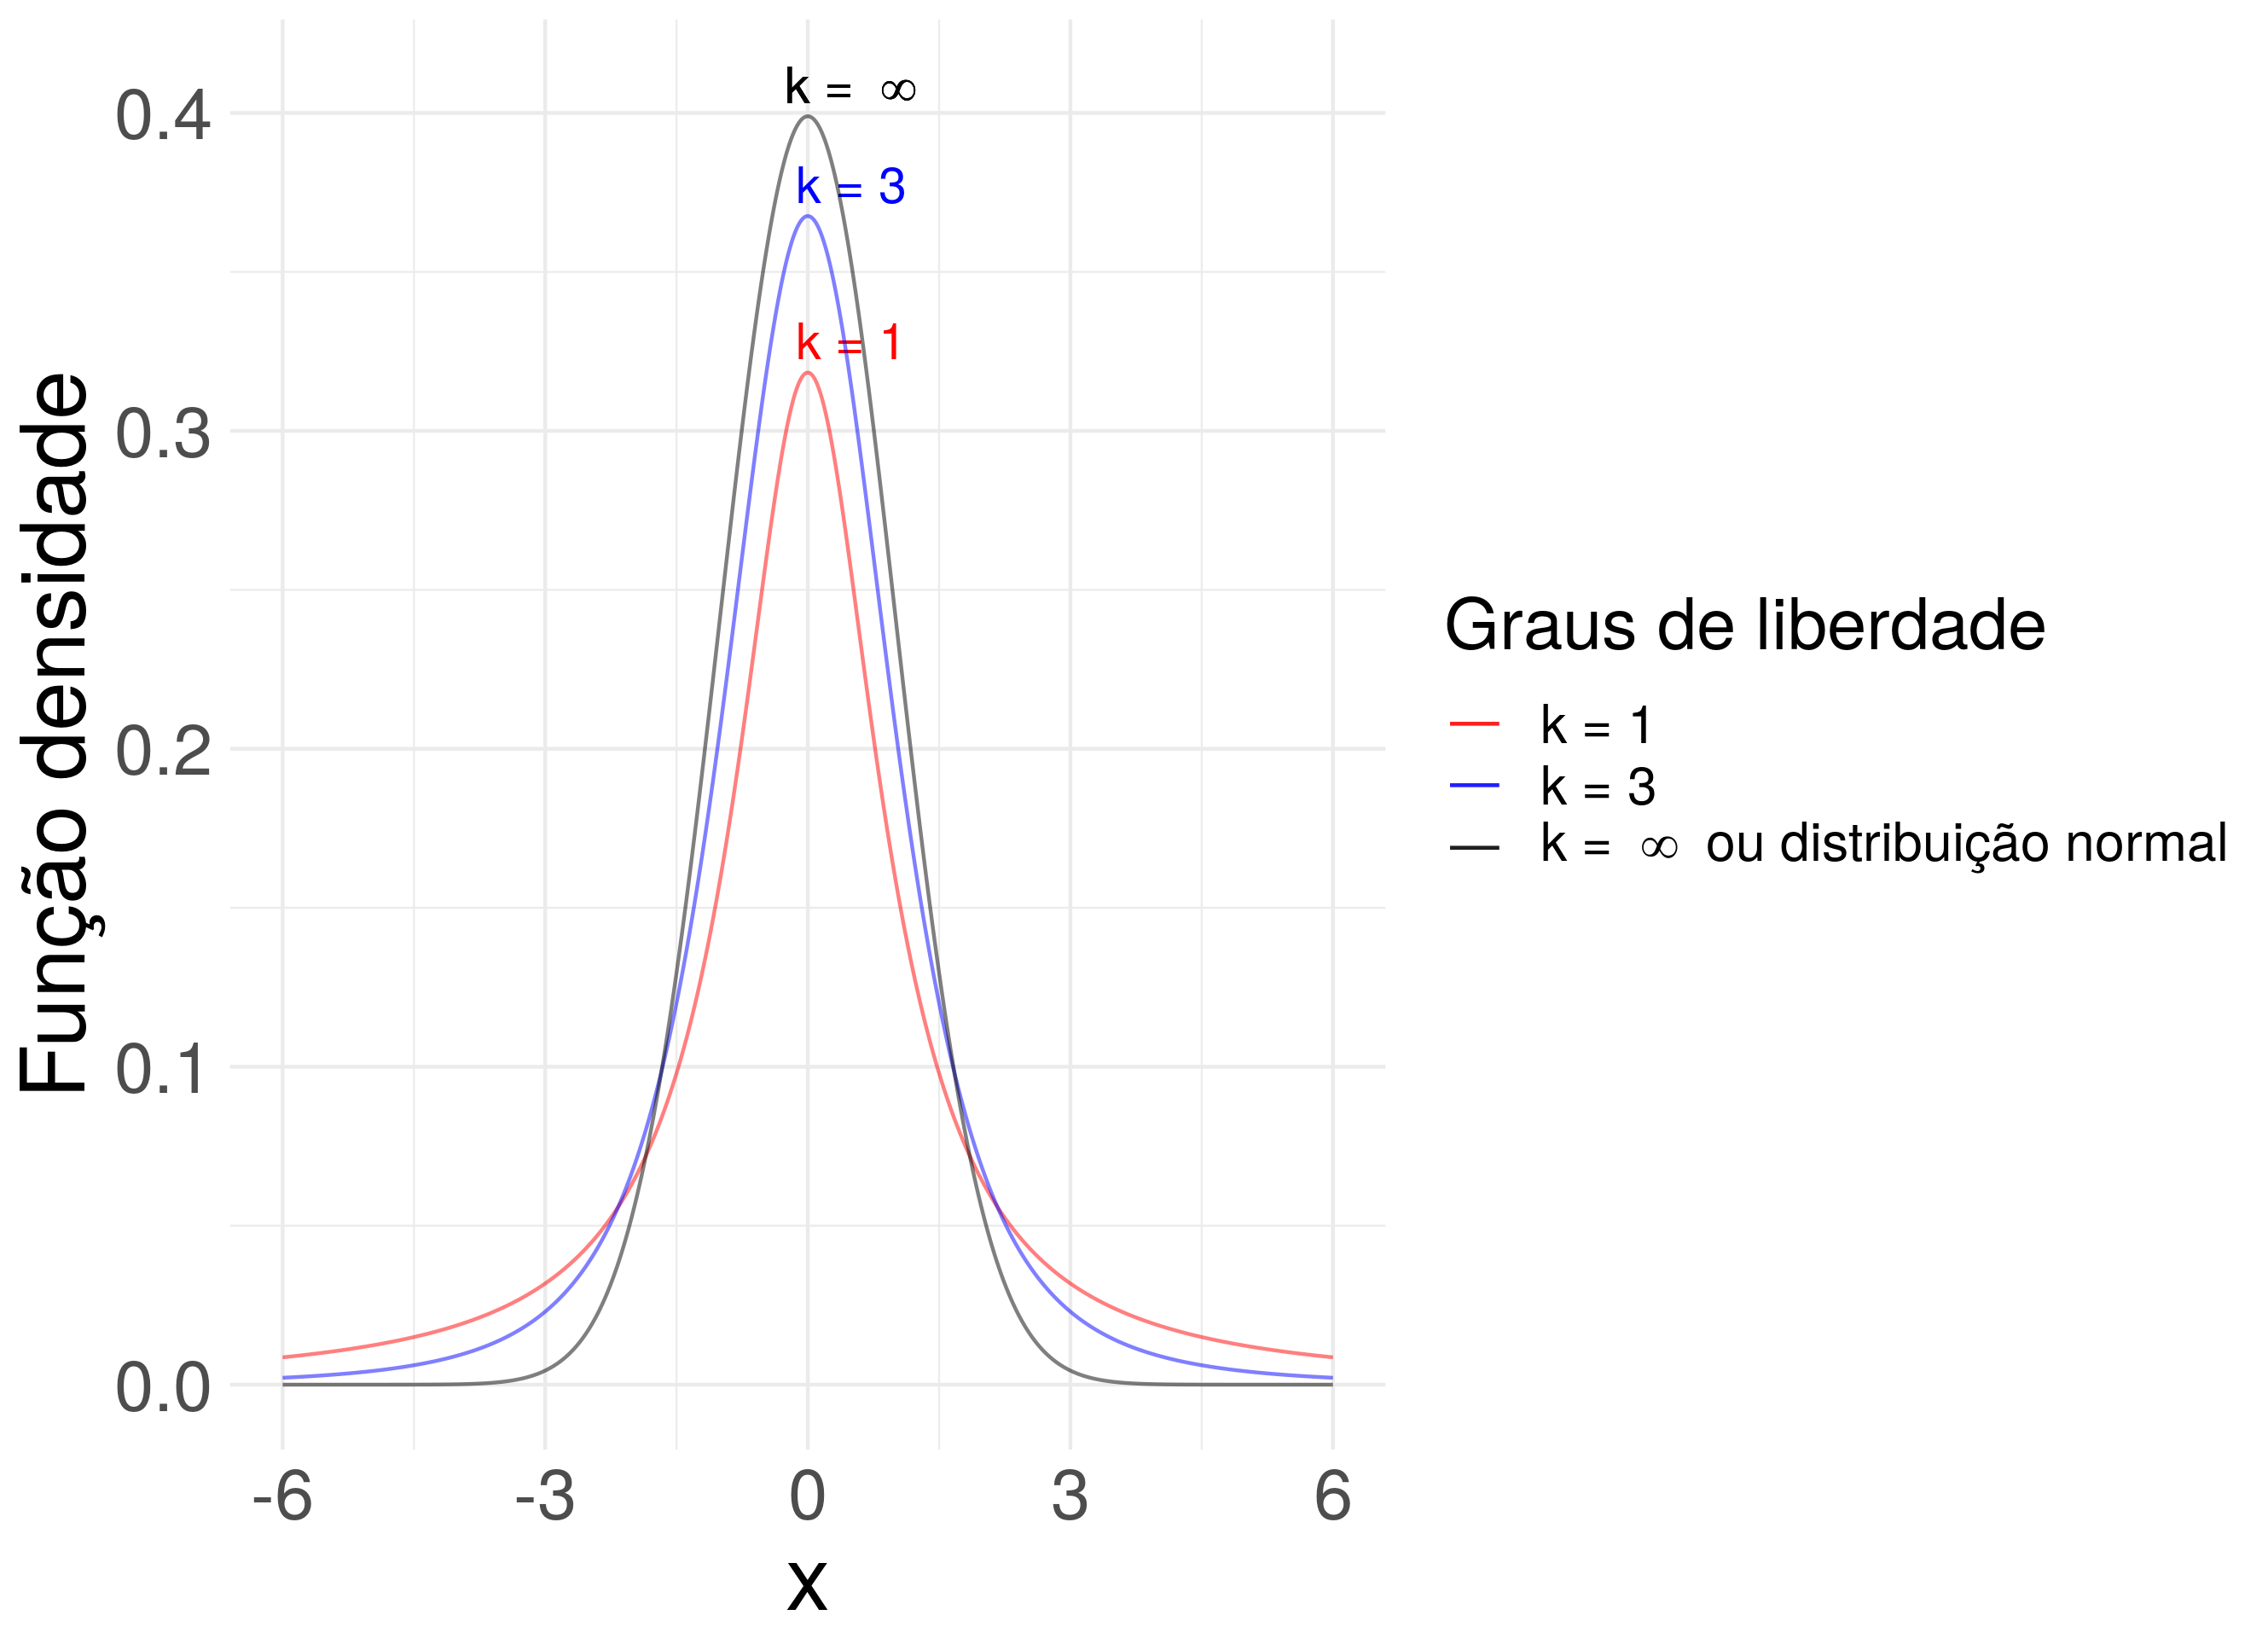
\includegraphics[width=9cm]{t-student.png}
	\end{figure}

\end{frame}

\begin{frame}{Estimação intervalar para média $\mu$\\ Distribuição normal com $\sigma^2$ desconhecida}
\Large

	Suponha que você sabe que a variável contínua $X$ com distribuição normal e não conhecemos o desvio padrão $\sigma$. Seja $x_1, \dots, x_n$ uma amostra de tamanho $n$ da variável $X$ com média $\bar{x} = \frac{x_1 + \dots + x_n}{n}$ e variância $s^2 = \frac{(x_1 - \bar{x})^2 + \dots + (x_n - \bar{x})^2}{n-1}$, então o intervalo de confiança com coeficiente de confiança $\gamma = 1-\alpha$ é dada por
	\begin{align*}
		IC(\mu, \gamma) = \left( \bar{x} - t_{1-\frac{\alpha}{2};n-1} \cdot  \dfrac{s}{\sqrt{n}}; \bar{x} + t_{1-\frac{\alpha}{2};n-1} \cdot  \dfrac{s}{\sqrt{n}} \right),
	\end{align*}
	em que $P\left( t_{n-1} \leq t_{1-\frac{\alpha}{2};n-1}  \right) = 1 - \dfrac{\alpha}{2}$, em que $t_{n-1}$ é a distribuição $t$-Student com $n-1$ graus de liberdade.
	
\normalsize
\end{frame}

\begin{frame}{Estimação intervalar para média $\mu$\\ Distribuição normal com $\sigma^2$ desconhecida}

\small
	\begin{block}{Exemplo}
		A força de compressão de um concreto é normalmente distribuída e um engenheiro civil precisa encontrar um intervalo de confiança para a força de compressão média e para isso coletou uma amostra com 12 espécimes de concreto e obteve a seguinte amostra: 2216, 2237, 2249, 2204, 2225, 2301, 2281, 2263, 2318, 2255, 2275, 2295. Use o coeficiente de confiança $\gamma = 0.99$.
		
	\end{block}
	\vfill

	\begin{block}{Solução}
		Primeiro calculamos o quantil da distribuição $t$-Student com $n-1$ com graus de liberdade através de $P(t_{n-1} \leq t_{1-\frac{\alpha}{2};n-1} ) = P(t_{11} \leq t_{0,995;11}) = 0,995$, então $t_{0,995;11} = 3,106$. A média e o desvio padrão são dadas por
		\begin{align*}
			\bar{x} = 2259,917 \mbox{ e } s = 35,56929.
		\end{align*}
		E o intervalo de confiança com coeficiente de confiança $\gamma = 0.99$ é 
		\begin{align*}
			IC(\mu, 99\%) &= \left( \bar{x} - t_{0,995;11} \dfrac{s}{\sqrt{n}}; \bar{x} + t_{0,995;11} \dfrac{s}{\sqrt{n}}  \right)\\
			&= \left( 2259,917 - 3,106 \cdot \dfrac{35,56929}{\sqrt{12}}; 2259,917 + 3,106 \cdot \dfrac{35,56929}{\sqrt{12}} \right)\\
			&= (2228,024; 2291,809)
		\end{align*}
		Ou seja, com coeficiente de confiança $\gamma=99\%$, a média populacional da força compressiva está entre $2228,024psi$ e $2291,809psi$.
	\end{block}
\normalsize

\end{frame}

\subsection{Intervalo unilateral de confiança para $\mu$}

\begin{frame}{Intervalo unilateral de confiança para $\mu$\\ Distribuição normal com $\sigma^2$ desconhecida}


Seja $x_1, \dots, x_n$ uma amostra aleatória de uma variável aleatória contínua com distribuição normal com média $\mu$ e variância desconhecida $\sigma^2$ e variância amostral $s^2 = \frac{(x_1 - \bar{x})^2 + \dots + (x_1 - \bar{x})^2}{n-1}$. 

\begin{block}{Limite superior de confiança}
	Ao nível de significância $\gamma=(1-\alpha)100\%$, o limite superior de confiança para média é dada por
	\begin{align*}
	\mu \leq \bar{x} + t_{1-\alpha;n-1} \frac{s}{\sqrt{n}},
	\end{align*}
	em que $P\left( t_{n-1} \leq t_{1-\alpha;n-1} \right) = 1-\alpha$, em que $t_{n-1}$ é uma variável aleatória com distribuição $t$-Student com $n-1$ graus de liberdade.
	
\end{block}

\begin{block}{Limite inferior de confiança}
	Ao nível de significância $\gamma=(1-\alpha)100\%$, o limite inferior de confiança para média é dada por
	\begin{align*}
	\bar{x} - t_{\alpha;n-1} \frac{s}{\sqrt{n}} \leq \mu,
	\end{align*}
	em que $P\left( t_{n-1} \leq t_{\alpha;n-1} \right) = \alpha$, em que $t_{n-1}$ é uma variável aleatória com distribuição $t$-Student com $n-1$ graus de liberdade.
\end{block}



\end{frame}

\begin{frame}{Intervalo unilateral de confiança para $\mu$}

\small
	
	\begin{block}{Exemplo}
		Uma marca de margarina foi analisada para determinar o nível (em porcentagem) de ácido graxo poliinsaturado. De estudos anteriores, os pesquisadores podem assumir a normalidade dos dados. Seis potes de margarina desta marca foi coletada com os seguintes níveis (em porcentagem) de ácido graxo poliinsaturado: 6,8; 17,2; 17,4; 16,9; 16,5; 17,1. Encontre um limite inferior para a porcentagem média de ácido graxo poliinsaturado com coeficiente de confiança $\gamma=95\%$.
	\end{block}

	\begin{block}{Solução}
		A média e o desvio padrão são dados por
		\begin{align*}
			\bar{x} = 16,98 \qquad s = 0,32,
		\end{align*}
		e o quantil $P(t_{n-1} \leq t_{\alpha; n-1}) = P(t_5 \leq t_{\alpha;5}) = 5\%$ da distribuição $t$-Student $k=n-1=5$, ou seja, $t_{0,05; 5}=-2,015$. Então,
		\begin{align*}
			IC(\mu, 95\%) &= \left(\bar{x} + t_{\alpha; n-1} \frac{s}{\sqrt{n}}; \infty\right)\\
			&= \left(16,98 - 2,015 \cdot \frac{0,32}{\sqrt{6}}; \infty\right)\\
			&= (16,71; \infty).
		\end{align*}
		Ou seja, com coeficiente de confiança $\gamma=95\%$, a média populacional da porcentagem de ácido graxo poliinsaturado nos potes de margarina é no mínimo $16,71$.
		
	\end{block}

\normalsize

\end{frame}

\section{Estimação intervalar para $\sigma^2$ para distribuição normal}

\large

\begin{frame}{Estimação intervalar para $\sigma^2$\\ Distribuição normal}

\begin{block}{Distribuição Qui-quadrado}
	Imagine que temos uma amostra $x_1, \dots, x_n$ de uma variável aleatória contínua $X$ com distribuição normal com  média $\mu$ e variância $\sigma^2$, e considere a variância amostral $s^2 = \frac{(x_1 - \bar{x})^2 + \dots + (x_n - \bar{x})^2}{n-1}$. Então a quantidade
	\begin{align*}
		X^2 = \dfrac{(n-1)s^2}{\sigma^2},
	\end{align*}
	tem distribuição amostral que chamamos de \textit{qui-quadrado} com $k=n-1>0$ graus de liberdade.
	\vfill

	
	Função densidade de probabilidade da distribuição qui-quadrado com $k>0$ graus de liberdade:
	\begin{align*}
		f(x) = \dfrac{1}{2^{\frac{k}{2}} \Gamma\left( \frac{k}{2} \right)} x^{\frac{k}{2} - 1} \exp\left(-\frac{x}{2} \right), \qquad x> 0.
	\end{align*}
	$\mu = k$ e $\sigma^2 = 2k$.
\end{block}
	
\end{frame}

\begin{frame}{Estimação intervalar para $\sigma^2$\\ Distribuição normal}

\begin{figure}[htbp]
	\centering
	\caption{Função de densidade.}
	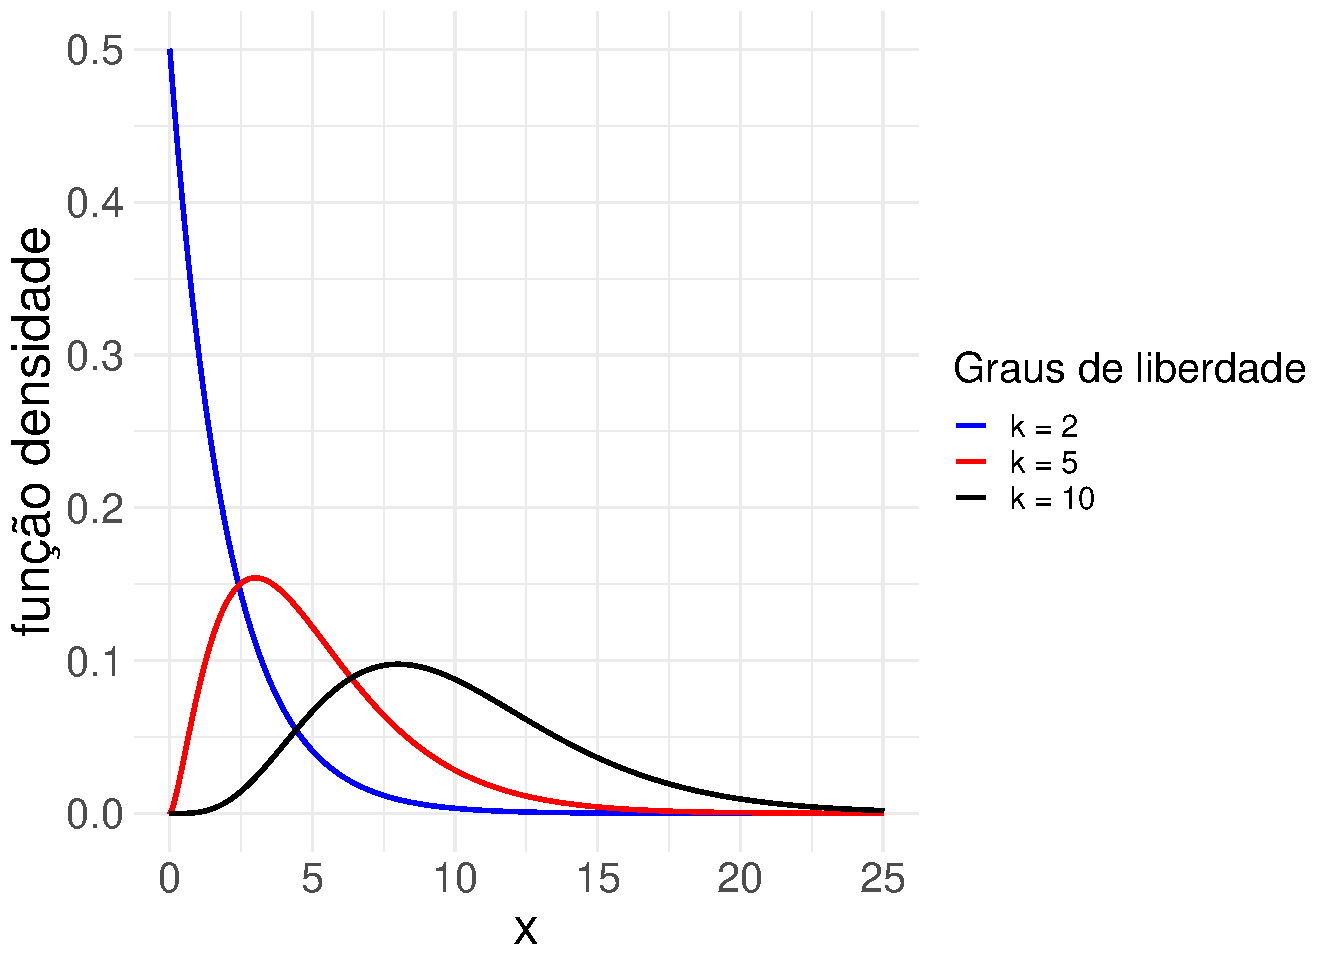
\includegraphics[width=8.5cm]{fd_qui_quadrado.pdf}
\end{figure}
	
\end{frame}


\begin{frame}{Estimação intervalar para $\sigma^2$\\ Distribuição normal}

\LARGE

Suponha que você sabe que a variável aleatória contínua $X$ com distribuição normal e não conhecemos o desvio padrão $\sigma$. Seja $x_1, \dots, x_n$ uma amostra de tamanho $n$ da variável $X$ com média $\bar{x} = \frac{x_1 + \dots + x_n}{n}$ e variância $s^2 = \frac{(x_1 - \bar{x})^2 + \dots + (x_n - \bar{x})^2}{n-1}$, então o intervalo de confiança para $\sigma^2$ com coeficiente de confiança $\gamma = 1-\alpha$ é dada por
\begin{align*}
IC(\sigma^2, \gamma) = \left( \frac{(n-1)s^2}{\chi^2_{1-\frac{\alpha}{2}; n-1}}; \frac{(n-1)s^2}{\chi^2_{\frac{\alpha}{2}; n-1}} \right)
\end{align*}
em que $P\left( \chi^2_{n-1} \leq \chi^2_{\frac{\alpha}{2}; n-1} \right) =  \dfrac{\alpha}{2}$ e $P\left( \chi^2_{n-1} \leq \chi^2_{\frac{1 - \alpha}{2}; n-1} \right) = 1 - \dfrac{\alpha}{2}$ , em que $\chi^2_{n-1}$ é a distribuição qui-quadrado com $n-1$ graus de liberdade.

\normalsize
\end{frame}

\begin{frame}{Intervalo de confiança para $\sigma^2$}

\small

\begin{block}{Exemplo}
	Um rebite está sendo construído para ser inserido em um buraco. Uma amostra aleatória com $n=15$ peças é selecionada, e o diâmetros dos buracos foram medidos. O desvio padrão amostral é dado por $s=0,008 ml$. Construa o intervalo de confiança para $\sigma^2$ com coeficiente de confiança $\gamma=99\%$.
\end{block}

\begin{block}{Solução}
	Primeiro encontramos os quantis da distribuição qui-quadrado $\chi^2_{n-1} = \chi^2_{15-1}=\chi^2_{14}$. 
	\begin{itemize}
		\item $P\left(\chi^2_{14} \leq \chi^2_{\frac{\alpha}{2}; 14}\right) = \frac{\alpha}{2} = \frac{0,01}{2} = 0,005$ e $\chi^2_{0,005; 14}=4,075$;
		\item $P\left(\chi^2_{14} \leq \chi^2_{1 - \frac{\alpha}{2}; 14}\right) = 1 - \frac{\alpha}{2} = 1 - \frac{0,01}{2} = 0,995$ e $\chi^2_{0,995; 14}=31,319$. 
	\end{itemize}
	Então,
	\begin{align*}
		IC(\sigma^2; \gamma) &= \left( \frac{(n-1)s^2}{\chi^2_{1-\frac{\alpha}{2}; 14}}; \frac{(n-1)s^2}{\chi^2_{\frac{\alpha}{2}; 14}} \right)\\
		&= \left( \frac{(15-1)0,008^2}{31,319}; \frac{(15-1)0,008^2}{4,075} \right) \\
		&= \left( 0,00003; 0,00022 \right).
	\end{align*}	
	Ou seja, com coeficiente de confiança $\gamma=99\%$, então a variância está entre $0,00003$ e $0,00022$.
	
\end{block}

\normalsize

\end{frame}

\subsection{Intervalo unilateral de confiança para $\sigma^2$}

\begin{frame}{Intervalo unilateral de confiança para $\sigma^2$}

\small

Seja $x_1, \dots, x_n$ uma amostra aleatória de uma variável aleatória contínua com distribuição normal com média $\mu$, variância desconhecida $\sigma^2$ e variância amostral $s^2 = \frac{(x_1 - \bar{x})^2 + \dots + (x_1 - \bar{x})^2}{n-1}$. 

\begin{block}{Limite superior de confiança}
	Ao nível de significância $\gamma=(1-\alpha)100\%$, o limite superior de confiança para variância é dada por
	\begin{align*}
	\sigma^2 \leq \frac{(n-1)s^2}{\chi^2_{\alpha; n-1}},
	\end{align*}
	em que $P\left( \chi^2_{n-1} \leq \chi^2_{\alpha; n-1} \right) = \alpha$, em que $\chi^2_{n-1}$ é uma variável aleatória com distribuição qui-quadrado com $n-1$ graus de liberdade.
	
\end{block}

\begin{block}{Limite inferior de confiança}
	Ao nível de significância $\gamma=(1-\alpha)100\%$, o limite inferior de confiança para média é dada por
	\begin{align*}
		\frac{(n-1)s^2}{\chi^2_{1-\alpha; n-1}} \leq \sigma^2,
	\end{align*}
	em que $P\left( \chi^2_{n-1} \leq \chi^2_{1-\alpha; n-1} \right) = 1-\alpha$, em que $\chi^2_{n-1}$ é uma variável aleatória com distribuição qui-quadrado com $n-1$ graus de liberdade.
\end{block}

\normalsize

\end{frame}

\begin{frame}{Intervalo unilateral de confiança para $\sigma^2$}

\normalsize

\begin{block}{Exemplo}
	A porcentagem de titânio numa liga de aço usada na construção de naves aeroespaciais tem distribuição normal, e um engenheiro coletou $51$ barras de aço com desvio padrão amostral $s=0,37$. Construa um limite superior para o desvio padrão populacional da porcentagem de titânio numa liga de aço com coeficiente de confiança $\gamma=95\%$.
\end{block}

\begin{block}{Solução}
	Primeiro encontramos o quantil, ou seja, $P\left( \chi^2_ {n-1} \leq \chi^2_{\alpha; n-1} \right) = P\left( \chi^2_ {50} \leq \chi^2_{0,05; 50} \right) = 0,05$ e $\chi^2_{0,05; 50} = 34,764$. Então, temos que
	\begin{align*}
		IC(\sigma^2; \gamma) &= \left( 0; \frac{(n-1)s^2}{\chi^2_{\alpha; n-1}} \right)\\
		&= \left( 0; \frac{50\cdot 0,37^2}{34,764} \right)\\
		&= \left(0; 0,197\right)
	\end{align*}
	Ou seja, com coeficiente de confiança $\gamma=95\%$, a variância populacional da porcentagem de titânio na liga de aço é no máximo $0,197$.
\end{block}

\normalsize

\end{frame}

\section{Estimação intervalar para $\mu$ para distribuição exponencial}

\begin{frame}{Estimação intervalar para $\mu$}
	
\LARGE

Suponha que você sabe que a variável contínua $X$ com distribuição exponencial e não conhecemos a média $\mu$ e taxa de decaimento $\lambda = \frac{1}{\mu}$. Seja $x_1, \dots, x_n$ uma amostra de tamanho $n$ da variável $X$ com média $\bar{x} = \frac{x_1 + \dots + x_n}{n}$, é possível provar que a distribuição da quantidade $2 \frac{1}{\mu} n \bar{x}$ tem distribuição qui-quadrado com $2n$ graus de liberdade. Então, o intervalo de confiança para $\mu$ com coeficiente de confiança $\gamma = (1-\alpha)100$, é dado por
\begin{align*}
	IC(\mu; \gamma) = \left( \frac{2 n \bar{x}}{\chi^2_{1-\frac{\alpha}{2}; 2n}}; \frac{2 n \bar{x}}{\chi^2_{\frac{\alpha}{2}; 2n}} \right),
\end{align*}
em que $P\left( \chi^2_{2n} \leq \chi^2_{\frac{\alpha}{2}; 2n} \right) = \frac{\alpha}{2}$ e $P\left( \chi^2_{2n} \leq \chi^2_{\frac{1-\alpha}{2}; 2n} \right) = 1- \frac{\alpha}{2}$, em que $\chi^2_{2n}$ tem distribuição qui-quadrado com $2n$ graus de liberdade.

\normalsize

\end{frame}

\begin{frame}{Estimação intervalar para $\mu$}

\footnotesize

\begin{block}{Exemplo}
	Um fabricante de lâmpadas afirma que a duração média, pelo menos, $20000$  horas. Um consumidor cético comprou 10 lâmpadas e verificou o tempo de vida de cada lâmpada. Os dados obtidos foram: 4272,61;  1464,02;  9765,54;  3308,58;  3237,83;   987,60;  4094,58; 17491,86;  4908,06 e  9403,13. Com coeficiente de confiança $\gamma=99\%$, este consumidor deve acreditar no fabricante de lâmpadas?
\end{block}

\begin{block}{Solução}
	Primeiro calculamos a média $\bar{x} = 5893,381$.
	
	Em seguida, calculamos os quantis da distribuição qui-quadrado:
	\begin{itemize}
		\item $P\left(\chi^2_{2n} \leq \chi^2_{\frac{\alpha}{2};2n}\right) = P\left(\chi^2_{20} \leq \chi^2_{\frac{0,01}{2};20}\right) = \frac{0,01}{2}$ e $\chi^2_{0,005;20} = 7,434$;
		\item $P\left(\chi^2_{2n} \leq \chi^2_{1-\frac{\alpha}{2};2n}\right) = P\left(\chi^2_{20} \leq \chi^2_{1-\frac{0,01}{2};20}\right) =1- \frac{0,01}{2}=0,995$ e $\chi^2_{0,995;20} = 39,997$.
	\end{itemize}
	Então, o intervalo de confiança para $\mu$ com coeficiente de confiança $\gamma=99\%$ é dada por
	\begin{align*}
		IC(\mu, \gamma) &= \left( \frac{2n \bar{x}}{\chi^2_{0,995;20}}; \frac{2n \bar{x}}{\chi^2_{0,005;20}}  \right)\\
		&= \left( \frac{2\cdot 10 \cdot 5893,381}{39,997}; \frac{2\cdot 10 \cdot 5893,381}{7,434}  \right)\\
		&= \left( 2.946,91; 15855,21 \right)
	\end{align*}
	Ou seja, com  coeficiente de confiança $\gamma=99\%$, o tempo médio de duração da lâmpada está entre $2.946,91$ e $15855,21$ horas.
\end{block}

\normalsize

\end{frame}

\subsection{Intervalo unilateral de confiança para $\mu$}

\begin{frame}{Intervalo unilateral de confiança para $\mu$\\ Distribuição exponencial com média $\mu$ e taxa de decaimento $\lambda=\frac{1}{\mu}$}

\small

Seja $x_1, \dots, x_n$ uma amostra aleatória de uma variável aleatória contínua com distribuição exponencial com média $\mu$ e e taxa de decaimento $\lambda=\frac{1}{\mu}$ e variância amostral $\bar{x} = \frac{x_1 + \dots + x_n}{n}$. 

\begin{block}{Limite superior de confiança}
	Ao nível de significância $\gamma=(1-\alpha)100\%$, o limite superior de confiança para média é dada por
	\begin{align*}
	\mu \leq \frac{2n \bar{x}}{\chi^2_{\alpha; 2n}},
	\end{align*}
	em que $P\left( \chi^2_{2n} \leq \chi^2_{\alpha; 2n} \right) = \alpha$, em que $\chi^2_{2n}$ é uma variável aleatória com distribuição qui-quadrado com $2n$ graus de liberdade.
	
\end{block}

\begin{block}{Limite inferior de confiança}
	Ao nível de significância $\gamma=(1-\alpha)100\%$, o limite inferior de confiança para média é dada por
	\begin{align*}
	\frac{2 n \bar{x}}{\chi^{2}_{1-\alpha;2n}} \leq \mu,
	\end{align*}
	em que $P\left( \chi^2_{2n} \leq \chi^{2}_{1-\alpha;2n} \right) = 1-\alpha$, em que $\chi^2_{2n}$ é uma variável aleatória com distribuição qui-quadrado com $2n$ graus de liberdade.
\end{block}

\normalsize

\end{frame}

\begin{frame}{Intervalo unilateral de confiança para $\mu$\\ Distribuição exponencial com média $\mu$ e taxa de decaimento $\lambda=\frac{1}{\mu}$}

\small

\begin{block}{Exemplo}
	Um fabricante afirma que o tempo de vida de um ventilador usado na montagem de computadores \textit{desktop} duram, em média, no mínimo 10.000 horas (conforme especificações de um órgão regulador). Este órgão regulador coletou 50 computadores do mercado e verificou quando tempo cada um dos ventiladores aguentaram e obteve uma média de 1953,063 horas. Ao nível de significância $\gamma=90\%$, o fabricante está cumprindo as especificações do regulador?
\end{block}

\begin{block}{Solução}
	Primeiro calculamos o quantil da distribuição qui-quadrado, ou seja, $P(\chi^2_{2n} \leq \chi_{\alpha;2n}^{2}) = P(\chi^2_{100} \leq \chi_{0,1;100}^{2}) = 0,9$ e $\chi_{0,1;100}^{2} = 82,358$. Então, temos que
	\begin{align*}
		IC(\mu, \gamma) &= \left( 0; \frac{2 n \bar{x}}{\chi_{0,1;100}^{2}} \right)\\
		&= \left( 0; \frac{2 \cdot 50\cdot 1953,063}{82,358} \right)\\
		&= \left( 0; 2380,536 \right).
	\end{align*}
	Ou seja, com coeficiente de confiança com $\gamma=90\%$, a média populacional de tempo de duração dos ventiladores não segue as especificações do regulador.
\end{block}

\normalsize

\end{frame}

\section{Intervalos de confiança para amostras grandes $n \geq 40$}

\subsection{Intervalo para proporção (Bernoulli)}

\begin{frame}{Intervalo de confiança para proporção $p$\\ Amostras grandes e distribuição Bernoulli}

\small

	Seja $x_1, \dots, x_n$ uma amostra de uma distribuição Bernoulli em que $n \geq 40$. Podemos aproximar a proporção $p$ por $\hat{p}=\frac{x_1 + \dots + x_n}{n}$. Usando o teorema central do limite, temos que a quantidade $\frac{\sqrt{n}(\hat{p} - p)}{p \cdot (1 - p)} $ tem distribuição normal padrão $ N(0, 1)$. Então o intervalo de confiança com coeficiente de confiança $\gamma=(1-\alpha)100\%$ seria dado por
	\begin{align*}
		IC(p; \gamma) = \left( -z_{1-\frac{\alpha}{2}} \frac{p\cdot (1-p)}{\sqrt{n}} + \hat{p}; z_{1-\frac{\alpha}{2}} \frac{p\cdot (1-p)}{\sqrt{n}} + \hat{p} \right).
	\end{align*}
	em que $\Phi(z_{1-\frac{\alpha}{2}}) = 1- \frac{\alpha}{2}$.
	Note que $p \cdot (1 - p) \leq \frac{1}{4}$, conforme ilustrado na Figura~\ref{fig:proportion}, e então
	\begin{align*}
	IC(p; \gamma) = \left( -z_{1-\frac{\alpha}{2}} \frac{1}{2\sqrt{n}} + \hat{p}; z_{1-\frac{\alpha}{2}} \frac{1}{2\sqrt{n}} + \hat{p} \right).
	\end{align*}
	
	\begin{figure}[htbp]
		\centering
		\caption{Ilustração da desigualdade $p \cdot (1-p) \leq \frac{1}{4}$. }
		\label{fig:proportion}
		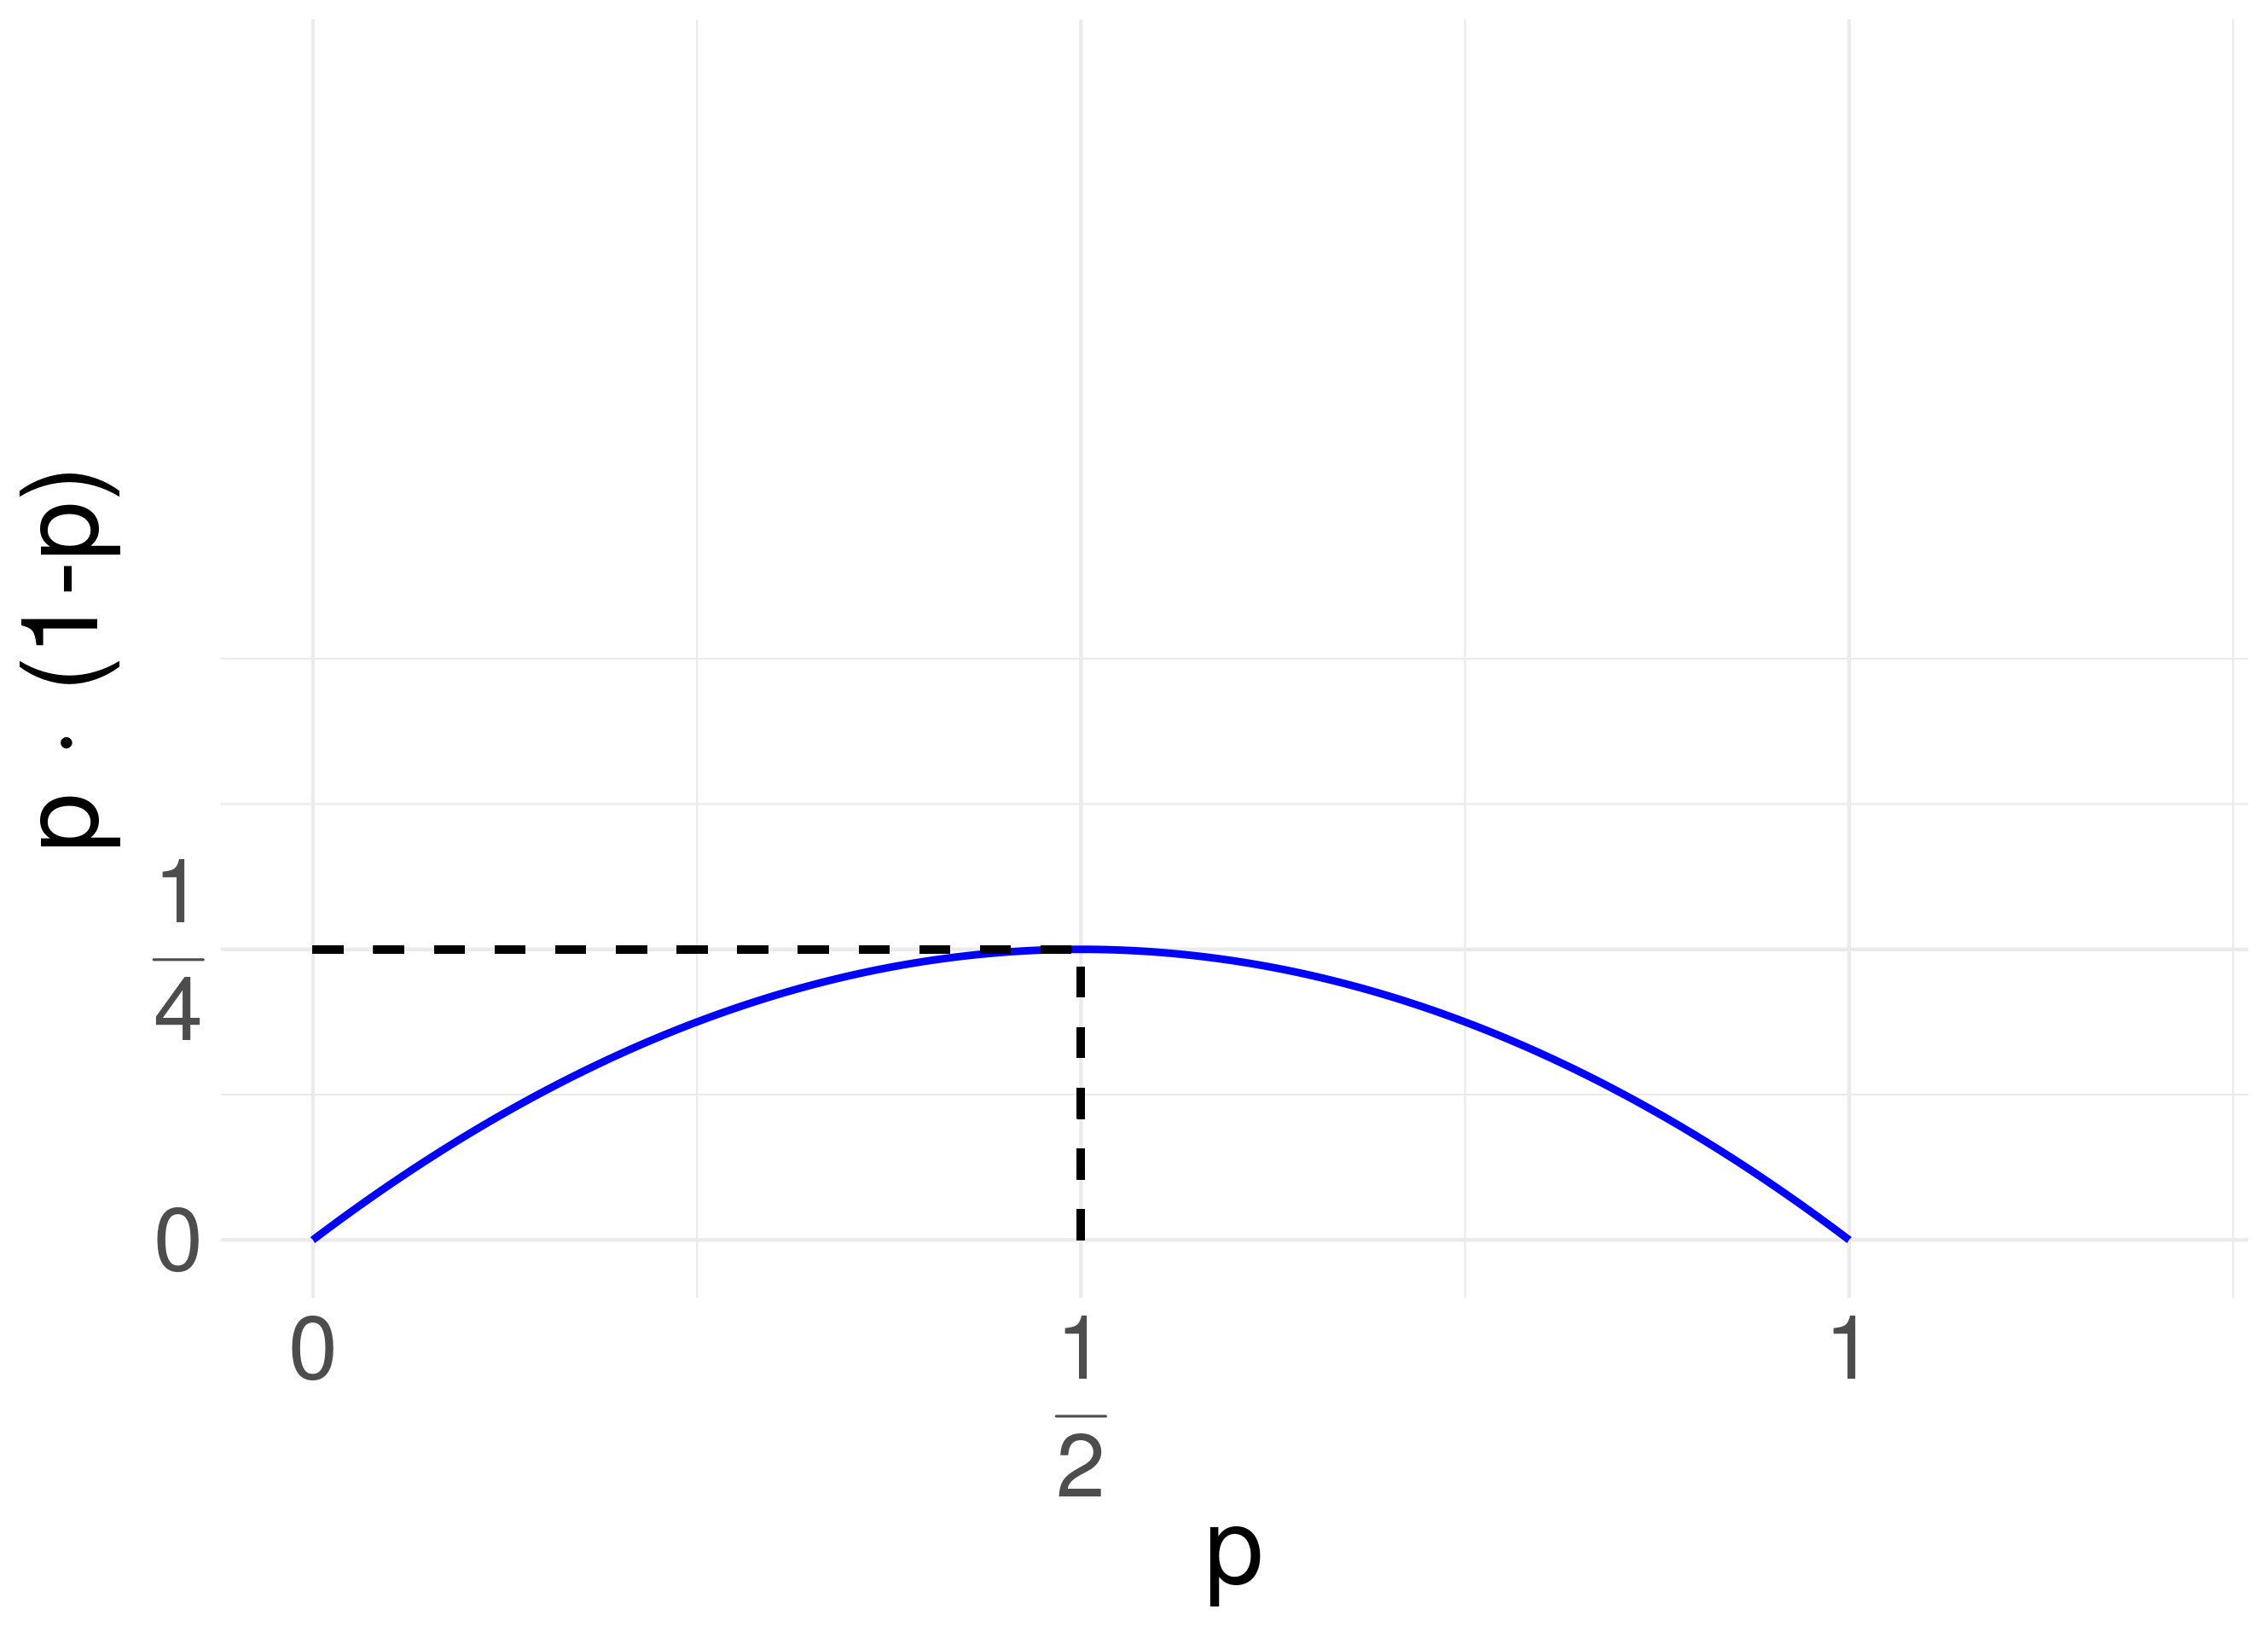
\includegraphics[width=4cm]{proportion.png}
	\end{figure}

\normalsize 

\end{frame}

\begin{frame}{Intervalo de confiança para proporção $p$\\ Amostras grandes e distribuição Bernoulli}

\small

\begin{block}{Exemplo}
	Uma equipe de qualidade quer determinar a proporção de circuitos integrados defeituosos produzidos por uma linha de produção. Uma amostra com $300$ circuitos é testada com $13$ circuitos defeituosos. Construa um intervalo de confiança para a proporção de circuitos defeituosos usando coeficiente de confiança $\gamma=90\%$.
\end{block}

\begin{block}{Solução}
	Primeiramente, calculamos a proporção de circuitos defeituosos: $\hat{p} = \frac{13}{300} = 0,043$. 
	
	Em seguida, encontramos o quantil da distribuição normal: $\Phi(z_{1-\frac{\alpha}{2}}) = 1 - \frac{\alpha}{2} = 0,95$ e $z_{1-\frac{\alpha}{2}} = 1,65$.
	
	Então, temos que
	\begin{align*}
		IC(p; \gamma) &= \left( - z_{1-\frac{\alpha}{2}} \frac{1}{2\sqrt{n}} + \hat{p}; z_{1-\frac{\alpha}{2}} \frac{1}{2\sqrt{n}} + \hat{p} \right) \\
		&=\left( -1,65 \frac{1}{2\sqrt{300}} + 0,043; 1,65 \frac{1}{2\sqrt{300}} + 0,043 \right)\\
		&= \left( -0,005; 0,091 \right) = (0; 0,091).
	\end{align*}
	Ou seja, com coeficiente de confiança $90\%$, a proporção de circuitos integrados defeituosos está entre $0$ e $0,091$.
\end{block}

\end{frame}

\subsection{Tamanho da amostra}

\begin{frame}{Escolha do tamanho da amostra}

\scriptsize

\begin{block}{Precisão da estimativa}
	Quando usamos $\hat{p} = \bar{x} = \frac{x_1 \dots + x_n}{n}$ para aproximar $p$, o erro $E = \lvert \hat{p} - p \rvert$ é menor ou igual a $ \frac{z_{1-\frac{\alpha}{2}} }{2\sqrt{n}}$ com coeficiente de confiança $\gamma = 100(1-\alpha)\%$.conforme  ilustrado na Figura~\ref{fig:intervalo_conf_prop}.
	
	\begin{figure}
		\centering
		\caption{Erro quando usamos $\hat{p}$ para aproximar $p$}
		\label{fig:intervalo_conf_prop}
		\begin{tikzpicture}
		\draw[->] (-4,0) -- (4,0);
		\filldraw[blue] (-2,0) circle (1.5pt);
		\node[below] at (-2, 0) {\tiny $l=\hat{p} - z_{1-\frac{\alpha}{2}}\frac{1}{2 \sqrt{n}}$};
		\filldraw[blue] (-1, 0) circle (1.5pt);
		\node[below] at (-1,0) {\tiny $p$};
		\filldraw[blue] (0,0) circle (1.5pt);
		\node[below] at (0,0) {\tiny $\hat{p}$};
		\filldraw[blue] (2, 0) circle (1.5pt);
		\node[below] at (2,0) {\tiny $u=\hat{p} + z_{1-\frac{\alpha}{2}}\frac{1}{2 \sqrt{n}}$};
		\draw[red] (-1, 0.2) -- (-1, 0.4);
		\draw[red] (0, 0.2) -- (0, 0.4);
		\draw[red] (-1, 0.3) -- (0, 0.3);
		\node[above, right, red] at (-1.2, 0.5) {\tiny $E = erro = \lvert p - \hat{p} \rvert$};
		\end{tikzpicture}
	\end{figure}
	Note que $z_\frac{\alpha}{2} \frac{1}{2\sqrt{n}}$ aumenta quando aumentamos $\gamma$ (ou diminuímos $\alpha$).  \textcolor{blue}{Dizemos que $z_\frac{\alpha}{2} \frac{1}{2\sqrt{n}}$ é a precisão da estimativa de $p$.}
\end{block}

\begin{block}{Tamanho da amostra}
	Quando fixamos $\gamma=1-\alpha$, então, para ter um erro máximo de $E$ ao aproximar $p$ por $\hat{p}$, o tamanho da amostra precisa ter no mínimo 
	\begin{align*}
	n = \left\lceil \left( \dfrac{z_{1-\frac{\alpha}{2}}  }{2E} \right)^2 \right\rceil,
	\end{align*}
	em que $\lceil x \rceil$ é ``$x$ é o primeiro inteiro depois de $x$'' e $E$ é o erro máximo tolerável especificado pelo pesquisador. Note que $\Phi\left(z_{1-\frac{\alpha}{2}}\right) = 1- \frac{\alpha}{2}$.
\end{block}

\normalsize

\end{frame}

\begin{frame}{Escolha do tamanho da amostra}
	
\normalsize
	
	\begin{block}{Exemplo}
		Um revendedor afirma que, em um pacote de sementes de alface, $95\%$ das sementes germinarão. Com coeficiente de confiança 99\%, qual o número mínimo de sementes que um órgão regulador precisa plantar para checar essa afirmação com erro máximo $E=1\%$?
		
	\end{block}

	\begin{block}{Solução}
		Primeiro calculamos o quantil da distribuição normal padrão $\Phi\left( z_{1-\frac{\alpha}{2}} \right) = \Phi\left( z_{0,995} \right) = 1 - \frac{\alpha}{2} = 0,995$ 	e $z_{0,995} = 2,58$. Então, o tamanho mínimo da amostra é dada por:
		\begin{align*}
			n &= \left\lceil \left( \frac{z_{1-\frac{\alpha}{2}}}{2 E} \right)^2 \right\rceil\\
			&= \left\lceil \left( \frac{2,58}{2 \cdot 0,01} \right)^2 \right\rceil\\
			&= \left\lceil 16,641 \right\rceil = 17.
		\end{align*}	
		Com coeficiente de confiança $95\%$ e erro máximo $E=0,01$, o tamanho mínimo de amostra é $\max(17, 40) = 40$ sementes.
	\end{block}

\normalsize

\end{frame}

\subsection{Intervalo unilateral de confiança para $p$}

\begin{frame}{Intervalo unilateral de confiança para $p$\\ Amostras grandes e distribuição Bernoulli}

\normalsize

Seja $x_1, \dots, x_n$ uma amostra aleatória de uma variável aleatória discreta com distribuição Bernoulli com proporção de sucesso $p$, em que $n \geq 40$. 

\begin{block}{Limite superior de confiança}
	Ao nível de significância $\gamma=(1-\alpha)100\%$, o limite superior de confiança para proporção é dada por
	\begin{align*}
		p \leq \hat{p} + z_{1-\alpha} \frac{1}{2\sqrt{n}},
	\end{align*}
	em que $\Phi(z_{1-\alpha}) = 1 - \alpha$, em que $\hat{p} = \frac{x_1 + \dots + x_n}{n}$.
	
\end{block}

\begin{block}{Limite inferior de confiança}
	Ao nível de significância $\gamma=(1-\alpha)100\%$, o limite inferior de confiança para proporção é dada por
	\begin{align*}
		z_\alpha \frac{1}{2 \sqrt{n}} + \hat{p} \leq p,
	\end{align*}
	em que $\Phi(z_\alpha) = \alpha$, em que $\hat{p} = \frac{x_1 + \dots + x_n}{n}$.
\end{block}

\normalsize

\end{frame}


\begin{frame}{Intervalo unilateral de confiança para $p$\\ Amostras grandes e distribuição Bernoulli}

\small

\begin{block}{Exemplo}
	O governo federal afirma que no mínimo 40\% dos poços artesianos da região nordeste tem água salobra. Um pesquisador da UFBA decide verificar essa afirmação, e analisou a água de 400 poços artesianos em diversos estados da região nordeste e 63 tiveram água salobra. Com coeficiente de confiança $\gamma=90\%$, qual a proporção máxima de poços artesianos com água salobra na região nordeste? O pesquisador concorda com o governo federal com coeficiente de confiança $\gamma=90\%$?
	
\end{block}

\begin{block}{Solução}
	Primeiro calculamos o quantil da distribuição normal padrão $\Phi\left( z_{1 - \alpha} \right) = \Phi\left( z_{0,90} \right) = 1-\alpha = 0,90$ e $z_{0,90} = 1,29$.
	
	
	A proporção de poços com água salobra é $\hat{p} = \frac{63}{400} = 0,16$.  Então, a proporção máxima de poços artesianos com água salobra é
	\begin{align*}
		IC(p, \gamma) &= \left( 0; \hat{p} + z_{1 - \alpha} \frac{1}{2 \sqrt{n}} \right)\\
		&= \left( 0; 0,16 + 1,29 \cdot \frac{1}{2 \cdot 20} \right)\\
		&= (0; 0,1923).
	\end{align*}
	Ou seja, com coeficiente de confiança $\gamma=90\%$, a proporção de poços artesianos é no máximo $19,23\%$. Ou seja, o pesquisador da UFBA discorda do governo federal e acredita que a proporção de poços artesianos é bem menor (no máximo $19,23\%$) com coeficiente de confiança $\gamma=90\%$.
\end{block}

\normalsize

\end{frame}

\subsection{Intervalo de confiança para $\mu$ para outras distribuições}

\begin{frame}{Intervalo de confiança para $\mu$\\ Amostras grandes e outras distribuições}

\huge

Seja $x_1, \dots, x_n$ uma amostra de tamanho $n$ de uma variável aleatória $X$ com média $\bar{x} = \frac{x_1 + \dots + x_n}{n}$ e $s^2 = \frac{(x_1 - \bar{x})^2 + \dots + (x_1 - \bar{x})^2}{n-1}$, em que $n \geq 40$. Então, o intervalo de confiança para $\mu$ com coeficiente de confiança $\gamma = (1-\alpha)100\%$ é dado por
\begin{align*}
IC(\mu; \gamma) = \left( \bar{x} -t_{1-\frac{\alpha}{2}; n-1} \frac{s}{\sqrt{n}}; \bar{x} + t_{1-\frac{\alpha}{2}; n-1} \frac{s}{\sqrt{n}} \right),
\end{align*}
em que $P\left( t_{n-1} \leq t_{1-\frac{\alpha}{2}; n-1} \right) = 1-  \frac{\alpha}{2}$, em que $t_{n-1}$ tem distribuição $t$-Student com $n-1$ graus de liberdade.

\normalsize

\end{frame}

\begin{frame}{Intervalo de confiança para $\mu$\\ Amostras grandes e outras distribuições}

\small

	\begin{block}{Exemplo}
		Imagine uma variável aleatória discreta com suporte $\chi=\{0,1,2,3,4,5\}$ e coletamos uma amostra com 15 valores: 1, 5, 5, 0, 1, 5, 5, 0, 1, 1, 1, 1, 4, 0 e 2. Construa um intervalo de confiança para média $\mu$ com coeficiente de confiança $\gamma=95\%$.
	\end{block}

	\begin{block}{Solução}
		Primeiro calculamos a média e o desvio padrão amostral: $\bar{x} = 2,13$ e $s= 2,03$. Em seguida, encontramos o quantil da distribuição $t$-Student com $n-1=15-1=14$ graus de liberdade: $P(t_{14} \leq t_{0,975;14})=1-\frac{\alpha}{2}=0,975$ e $t_{0,975;14} =2,145$. Então o intervalo de confiança para $\mu$ é dado por
		\begin{align*}
			IC(\mu, \gamma) &= \left( -t_{1-\frac{\alpha}{2};n-1} \frac{s}{\sqrt{n}} + \bar{x}; t_{1-\frac{\alpha}{2};n-1} \frac{s}{\sqrt{n}} + \bar{x} \right)\\
			&= \left( -t_{0,975;14} \frac{s}{\sqrt{n}} + \bar{x}; t_{0,975;14} \frac{s}{\sqrt{n}}  + \bar{x} \right)\\
			&= \left( -2,145 \frac{2,03}{\sqrt{15}} + 2,13; 2,145 \frac{2,03}{\sqrt{15}} + 2,13 \right)\\
			&= \left( 1,01; 3,25 \right).
		\end{align*}  
		Ou seja, com coeficiente de confiança $\gamma=95\%$, a média $\mu$ está entre $1,01$ e $3,25$.
		
	\end{block}

\normalsize 
\end{frame}

\subsection{Intervalo unilateral de confiança para $\mu$ para outras distribuições}

\begin{frame}{Intervalo unilateral de confiança para $\mu$\\ Amostras grandes e outras distribuições}

\normalsize

Seja $x_1, \dots, x_n$ uma amostra aleatória de uma variável aleatória $X$, em que $n \geq 40$.

\begin{block}{Limite superior de confiança}
	Ao nível de significância $\gamma=(1-\alpha)100\%$, o limite superior de confiança para média é dada por
	\begin{align*}
	\mu \leq \bar{x} + t_{1-\alpha;n-1} \frac{s}{\sqrt{n}},
	\end{align*}
	em que $P(t_{n-1} \leq t_{1-\alpha;n-1}) = 1 - \alpha$, em que $t_{n-1}$ é a distribuição $t$-Student com $n-1$ graus de liberdade.
	
\end{block}

\begin{block}{Limite inferior de confiança}
	Ao nível de significância $\gamma=(1-\alpha)100\%$, o limite inferior de confiança para média é dada por
	\begin{align*}
	\bar{x} + t_{\alpha;n-1} \frac{s}{\sqrt{n}} \leq \mu,
	\end{align*}
	em que $P(t_{n-1} \leq t_{\alpha;n-1}) = \alpha$, em que $t_{n-1}$ é a distribuição $t$-Student com $n-1$ graus de liberdade.
\end{block}

\normalsize

\end{frame}

\begin{frame}{Intervalo unilateral de confiança para $\mu$\\ Amostras grandes e outras distribuições}

\normalsize

\begin{block}{Exemplo}
	Um gerente de uma central de \textit{call center} 	está interessado em estimar o número máximo, em média, de chamadas que a central recebe. Com esse fim, o gerente contou quantas ligações a central recebeu em 20 dias úteis: 94, 98, 109, 102,  78, 105, 102,  97,  91,  95, 103,  93, 129, 115, 114, 110,  90, 103, 106 e 121. Com coeficiente de confiança $\gamma=99\%$, qual o número máximo, em média, de ligações que a central de \textit{call center} recebe em um dia útil?
\end{block}

\begin{block}{Solução}
	Primeiro calculamos a média e o desvio padrão amostral: $\bar{x} = 102,75$ e $s = 11,72$. Em seguida, encontramos o quantil da distribuição $t$-Student com $n-1=20-1=19$ graus de liberdade: $P(t_{19} \leq t_{0,99; 19}) = 0,99$ e $t_{0,99; 19} = 2,539$. Então o intervalo de confiança para $\mu$ é dado por
	\begin{align*}
	IC(\mu, \gamma) &= \left( 0; t_{1-\alpha;n-1} \frac{s}{\sqrt{n}} + \bar{x} \right)= \left(0; t_{0,99;19} \frac{s}{\sqrt{n}}  + \bar{x} \right) \\
	&= \left( 0; 2,359 \frac{11,72}{\sqrt{15}} + 102,75 \right) = \left( 0; 109,89 \right).
	\end{align*} 
	Ou seja, com coeficiente de confiança $\gamma=99\%$, o número máximo de chamadas que chegam, em média, é 110 chamadas.
	
\end{block}
\normalsize

\end{frame}

\section{Roteiro para construir intervalo de confiança}

\begin{frame}{Resumo para construir intervalo de confiança}

{\tiny%\fontsize{5}{5}\selectfont

\begin{table}[htbp]
	\centering
	\begin{tabular}{l|c|c|c}
		\toprule[0.05cm]
		Distribuição & Parâmetro & Intervalo  & Quantil \\ \midrule[0.05cm]
		Normal  & $\mu$ & $  IC(\mu, 1-\alpha) = \left(-z_{1-\frac{\alpha}{2}} \frac{\sigma}{\sqrt{n}} + \bar{x}; z_{1-\frac{\alpha}{2}} \frac{\sigma}{\sqrt{n}} + \bar{x} \right)$  & $\Phi\left(z_{1-\frac{\alpha}{2}}\right) = 1 - \frac{\alpha}{2}$ \\ 
		 $\sigma^2$ conhecido &  & $IC(\mu, 1-\alpha) = \left(z_{\alpha} \frac{\sigma}{\sqrt{n}} + \bar{x} ;\infty \right)$  & $\Phi\left(z_\alpha\right) = \alpha$ \\ 
		&  & $IC(\mu, 1-\alpha) = \left(-\infty; z_{1-\alpha}  \frac{\sigma}{\sqrt{n}} + \bar{x}\right)$  & $\Phi\left( z_{1-\alpha} \right) = 1 - \alpha$ \\ \midrule
		Normal  & $\mu$ & $IC(\mu, 1-\alpha) = \left( -t_{1-\frac{\alpha}{2}; n-1} \frac{s}{\sqrt{n}} + \bar{x}; t_{1-\frac{\alpha}{2}; n-1} \frac{s}{\sqrt{n}} + \bar{x} \right)$  & $P\left(t_{n-1} \leq t_{1-\frac{\alpha}{2}; n-1}\right) = 1 - \frac{\alpha}{2}$ \\ 
		&  & $IC(\mu, 1-\alpha) = \left( t_{\alpha; n-1} \frac{s}{\sqrt{n}} + \bar{x}; \infty \right)$  & P$\left(t_{n-1} \leq t_{\alpha; n-1}\right) =  \alpha$ \\ 
		&  & $IC(\mu, 1-\alpha) = \left( -\infty; t_{1-\alpha; n-1} \frac{s}{\sqrt{n}} + \bar{x}\right)$  & P$\left(t_{n-1} \leq t_{1-\alpha; n-1}\right) = 1- \alpha$ \\ \midrule
		Normal & $\sigma^2$ & $IC(\sigma^2; 1-\alpha) = \left( \frac{(n-1)s^2}{\chi^2_{1-\frac{\alpha}{2}; n-1}}; \frac{(n-1)s^2}{\chi^2_{\frac{\alpha}{2}; n-1}}  \right)$  & Vide ii. \\ 
		 &  & $IC(\sigma^2; 1-\alpha) = \left(\frac{(n-1)s^2}{\chi^2_{1-\alpha; n-1}}; \infty  \right)$  & $P\left( \chi^2_{n-1} \leq \chi^2_{1-\alpha; n-1} \right) = 1-\alpha$ \\ 
		 &  & $IC(\sigma^2; 1-\alpha) = \left(0; \frac{(n-1)s^2}{\chi^2_{\alpha; n-1}} \right)$  & $P\left( \chi^2_{n-1} \leq \chi^2_{\alpha; n-1} \right) = \alpha$ \\ \bottomrule[0.05cm]
	\end{tabular}
\end{table}
\begin{enumerate}[i.]
	\item $n$ é o tamanho da amostra;
	\item $P\left( \chi^2_{n-1} \leq \chi^2_{\frac{\alpha}{2};n-1} \right) = \frac{\alpha}{2}$ e $P\left( \chi^2_{n-1} \leq \chi^2_{1-\frac{\alpha}{2};n-1} \right) = 1- \frac{\alpha}{2}$.
\end{enumerate}
}


\end{frame}

\begin{frame}{Resumo para construir intervalo de confiança}

{\tiny
	
	\begin{table}[htbp]
		\centering
		\begin{tabular}{l|c|c|c}
			\toprule[0.05cm]
			Distribuição & Parâmetro & Intervalo  & Quantil \\ \midrule[0.05cm]
			Exponencial  & $\mu$ & $  IC(\mu, 1-\alpha) = \left( \chi^2_{1-\frac{\alpha}{2};2n} \cdot  \dfrac{1}{2n\bar{x}}; \chi^2_{\frac{\alpha}{2};2n} \cdot \dfrac{1}{2n\bar{x}} \right)$  & Vide ii. \\ 
			 &  & $IC(\mu, 1-\alpha) = \left( \chi^2_{1-\alpha;2n} \cdot  \dfrac{1}{2n\bar{x}} ;\infty \right)$  & $P\left( \chi^2_{2n} \leq \chi^2_{1-\alpha;2n}  \right)=1-\alpha$ \\ 
			&  & $IC(\mu, 1-\alpha) = \left(0; \chi^2_{\alpha;2n} \cdot  \dfrac{1}{2n\bar{x}} \right)$  & $P\left( \chi^2_{2n} \leq \chi^2_{\alpha;2n}  \right)=\alpha$ \\ \midrule
			Bernoulli  & $p$ & $IC(p, 1-\alpha) = \left( -z_{1-\frac{\alpha}{2}}\dfrac{1}{2\sqrt{n}} + \hat{p}; z_{1-\frac{\alpha}{2}}\dfrac{1}{2\sqrt{n}} + \hat{p} \right)$  & $\Phi\left( z_{1-\frac{\alpha}{2}} \right) = 1 - \frac{\alpha}{2}$ \\ 
			$n \geq 40$ &  & $IC(p, 1-\alpha) = \left( z_{\alpha} \dfrac{1}{2 \sqrt{n}} + \hat{p}; 1 \right)$  & $\Phi\left( z_\alpha \right) = \alpha$ \\ 
			&  & $IC(p, 1-\alpha) = \left( 0; z_{1-\alpha} \dfrac{1}{2 \sqrt{n}} + \hat{p} \right)$  & $\Phi\left( z_{1-\alpha} \right) = 1 - \alpha$ \\ \midrule
			Outras distribuições & $\mu$ & $IC(\mu; 1-\alpha) = \left( -t_{\frac{\alpha}{2}; n-1} \dfrac{s}{\sqrt{n}} + \bar{x}; t_{\frac{\alpha}{2}; n-1} \dfrac{s}{\sqrt{n}} + \bar{x} \right)$  & $P\left( t_{n-1} \leq t_{\frac{\alpha}{2}; n-1} \right) = 1- \frac{\alpha}{2}$  \\ 
			$n \geq 40$ &  & $IC(\mu; \gamma) = \left(t_{\alpha; n-1} \dfrac{s}{\sqrt{n}} + \bar{x}; \infty  \right)$  & $P\left( t_{n-1} \leq t_{\alpha; n-1} \right) = \alpha$ \\ 
			&  & $IC(\sigma^2; \gamma) = \left(-\infty; t_{1-\alpha; n-1} \dfrac{s}{\sqrt{n}} + \bar{x} \right)$  & $P\left( t_{n-1} \leq t_{1-\alpha; n-1} \right) = 1 - \alpha$ \\ \bottomrule[0.05cm]
		\end{tabular}
	\end{table}
	\begin{enumerate}[i.]
		\item $n$ é o tamanho da amostra;
		\item $P\left( \chi^2_{2n} \leq \chi^2_{\frac{\alpha}{2};2n} \right) = \frac{\alpha}{2}$ e $P\left( \chi^2_{2n} \leq \chi^2_{1-\frac{\alpha}{2};2n} \right) = 1- \frac{\alpha}{2}$.
	\end{enumerate}
}


\end{frame}


%
%\section{Distribuição Bernoulli}
%
%\begin{frame}{}
%
%{\scriptsize
%\begin{block}{Intervalo de confiança}
% Considere $x_1, \dots, x_n$ valores observados de uma variável aleatória com $X \sim Bernoulli(p)$. Então o intervalo de confiança para $p$ é dado por 
% \begin{align*}
%  IC(p, \gamma) = \left( -\dfrac{z_{\gamma}}{2 \cdot \sqrt{n}} + \hat{p}; \dfrac{z_{\gamma}}{2 \cdot \sqrt{n}} + \hat{p}\right),
% \end{align*} 
% em que $z_\gamma$ é encontrado através de $\Phi(z_\gamma) = \dfrac{1+\gamma}{2}$ e $n$ é o tamanho da amostra.
%\end{block}
%
%\begin{block}{Exemplo}
%   Em uma pesquisa de intenção de votos para uma possível eleição geral e direta em outubro, o IBOPE entrevistou 1000 pessoas e 40\% pessoas afirmaram Lula não deveria ser candidato. Com coeficiente de confiança $99\%$,
% qual o intervalo de confiança para a verdadeira de proporção de eleitores que não desejam que Lula seja candidato na eleição 2018?
% \vfill 
% 
% \textbf{Solução: }
% \begin{itemize}
%  \item $\Phi(z_{\gamma}) = \dfrac{1+\gamma}{2} = \dfrac{1+0,99}{2} = 0,995$ e $z_{\gamma} = 2,58$;
%  \item \begin{align*}
%	  IC(p; 99\%) &= \left( - \dfrac{z_{\gamma}}{2\sqrt{n}} + \hat{p}; \dfrac{z_{\gamma}}{2\sqrt{n}} + \hat{p} \right)\\
%	  &=\left( -\dfrac{2,58}{2\sqrt{1000}} + 0,4;\dfrac{2,58}{2\sqrt{1000}} + 0,4 \right) = (0,36; 0,44).
%        \end{align*} 
% \end{itemize} 
% Ou seja, a proporção verdadeira de eleitores que não desejam que Lula seja candidato está entre 36\% e 44\% com coeficiente de confiança 99\%.
%\end{block} 
%}
%\end{frame}
%% 
%%  \begin{frame}{Exemplo}
%%  Em uma pesquisa de intenção de votos para uma possível eleição geral e direta em outubro, o IBOPE entrevistou 1000 pessoas e 40\% pessoas afirmaram Lula não deveria ser candidato. Com coeficiente de confiança $99\%$,
%%  qual o intervalo de confiança para a verdadeira de proporção de eleitores que não desejam que Lula seja candidato na eleição 2018?
%%  \vfill 
%%  
%%  \textbf{Solução: }
%%  \begin{itemize}
%%   \item $\Phi(z_{\frac{\gamma}{2}}) = \dfrac{1+\gamma}{2} = \dfrac{1+0,99}{2} = 0,995$;
%%   \item \begin{align*}
%% 	  IC(p; 99\%) &= \left( - \dfrac{z_{\frac{\gamma}{2}}}{2\sqrt{n}} + \hat{p}; \dfrac{z_{\frac{\gamma}{2}}}{2\sqrt{n}} + \hat{p} \right)\\
%% 	  &=\left( -\dfrac{2,58}{2\sqrt{100}} + 0,4;\dfrac{2,58}{2\sqrt{100}} + 0,4 \right) = (0,36; 0,44).
%%         \end{align*} 
%%  \end{itemize}
%%  
%%  Ou seja, a proporção verdadeira de eleitores que não desejam que Lula seja candidato está entre 36\% e 44\% com coeficiente de confiança 99\%.
%% \end{frame}
%
%\section{Distribuição Poison}
%
%\begin{frame}{}
%
%{\scriptsize
% Considere $x_1, \dots, x_n$ valores observados de uma variável aleatória com $X_i \sim Poison(\lambda)$, então o intervalo de confiança com coeficiente de confiança é dada por
% \begin{align*}
%  IC(\lambda, \gamma) &= (\lfloor a \rfloor, \lceil b \rceil)
% \end{align*}
% em que 
% \begin{align*}
%  a &= \dfrac{1}{n} \left[ n \bar{x} + \dfrac{2 z_{\gamma}^2 +1 }{6} -  \dfrac{1}{2} - \sqrt{z_{\gamma}^2 \left( n\bar{x} -\frac{1}{2} + \frac{z_{\gamma}^2 + 2}{19} \right) }  \right]\\
%  b &= \dfrac{1}{n} \left[ n \bar{x} + \dfrac{2 z_{\gamma}^2 +1 }{6} +  \dfrac{1}{2} + \sqrt{z_{\gamma}^2 \left( n\bar{x} +\frac{1}{2} + \frac{z_{\gamma}^2 + 2}{19} \right) }  \right]
% \end{align*}
%em que 
%\begin{itemize}
% \item $\Phi(z_{\gamma}) = \dfrac{1+\gamma}{2}$ e $\gamma$ é o coeficiente de contingência;
% \item $\lceil x \rceil$ é a função ``arredonda para cima'', ou seja, ``o próximo número inteiro'';
% \item $\lfloor x \rfloor$ é a função ``arredonda para baixo'', ou seja, ``o número inteiro anterior''.
%\end{itemize}
%\begin{figure}[htbp]
%  \centering
%  \caption{Ilustração das funções $\lfloor x \rfloor$ e $\lceil x \rceil$.}
%  \begin{tikzpicture}[scale = 0.5]
%   \draw (0,0) -- (4,0);
%   \draw[black,fill=black] (1,0) circle (.25ex);
%   \draw[black,fill=black] (3,0) circle (0.25ex);
%   \node[below] at (1,0) {$\lfloor 1,2 \rfloor$};
%   \node[below] at (3,0) {$\lceil 1,2 \rceil$};
%   \node[above] at (1,0) {$1$};
%   \node[above] at (3,0) {$2$};
%   \draw[blue] (2,-1) -- (2,1);
%   \node[blue, below] at (2,-1) {$1,2$};
%  \end{tikzpicture}
%\end{figure}
%Para maiores detalhes, consulte: \textit{``Confidence intervals for the mean of a Poison distribuição: a review.''}
%}
%\end{frame}
%
%\begin{frame}{Exemplo}
%  
%  Um enfermeiro anotou o número de atendimentos de uma unidade básica de saúde por 15 dias úteis obtendo os valores da tabela \ref{fig:ci_pois}.
%  {\scriptsize
%  \begin{table}[ht]
%\centering
%\begin{tabular}{l|ccccccccccccccc}
%  \toprule[0.05cm]
%Número de atendimentos & 11 & 11 & 9 & 10 & 9 & 11 & 13 & 12 & 9 & 8 & 11 & 4 & 11 & 7 & 8 \\ 
%   \bottomrule[0.05cm]
%\end{tabular}
%\caption{Número de atendimento em dia útil.} 
%\label{fig:ci_pois}
%\end{table}
%}
%Com coeficiente de confiança $\gamma=99\%$, construa um intervalo de confiança para o número médio de atendimento nesta unidade básica de saúde.
%\vfill
%
%{\small
%\textbf{Solução: } A média é $\bar{x} = 9,6$ e $\Phi(z_{\gamma}) = \dfrac{1+\gamma}{2}=0,995$, ou seja, $z_{\gamma} = 2,58$. Então, 
%\begin{align*}
% IC(\lambda, 99\%) &= \left( \dfrac{1}{15}(15\cdot 9,6 + \dfrac{2 \cdot 2,58^2+1}{6} -0,5 - \sqrt{2,58^2(15\cdot 9,6 -0.5 +\dfrac{2,58^2+2}{18}) };  \right.\\
%&\left. \dfrac{1}{15}(15\cdot 9,6 + \dfrac{2 \cdot 2,58^2+1}{6} +0,5 + \sqrt{2,58^2(15\cdot 9,6 +0.5 +\dfrac{2,58^2+2}{18}) } \right)
%\end{align*}
%}
%
%e $IC(\lambda, 99\%) = (\lfloor 7,66 \rfloor; \lceil 11,83 \rceil)=(7,12)$, ou seja, com coeficiente de confiança $99\%$ o número médio de pacientes atendidos na UBS está entre 7 e 12 pacientes.
%\end{frame}
%
%
%\section{Distribuição exponencial}
% 
%\begin{frame}{}
% Assuma que $x_1, \dots, x_n$ sao valores observados de uma variável aleatória $X \sim Exp(\alpha)$. 
% 
%%  Relembre que $\dfrac{\bar{X}-\frac{1}{\alpha}}{\sqrt{ \frac{1}{n \cdot \alpha^2} }} \sim Normal(0,1)$, ou seja, $ \sqrt{n}(\alpha \bar{X} - 1) \sim Normal(0,1)$.
% 
% Seja $\gamma \in (0,1)$ e $z_{\gamma}$ tal que $\Phi(z_{\gamma}) = \dfrac{1+\gamma}{2}$, então o seguinte intervalo de confiança para $\alpha$ é 
%\begin{align*}
% IC(\alpha; \gamma) = \left( \dfrac{\frac{-z_{\gamma}}{\sqrt{n}} +1 }{\bar{X}};\dfrac{\frac{z_{\gamma}}{\sqrt{n}} +1 }{\bar{X}} \right)
%\end{align*}
%e o intervalo de confiança para a média $\mu$ é 
%\begin{align*}
% IC(\mu; \gamma) = \left( \dfrac{\bar{X}}{\dfrac{ z_{\gamma} }{\sqrt{n}} +1}  ; \dfrac{\bar{X}}{ -\dfrac{ z_{\gamma} }{\sqrt{n}} +1} \right)
%\end{align*}
%
%\end{frame}
%
%\begin{frame}{Exemplo}
%
%{\scriptsize
% Uma induśtria fabrica lâmpadas que ficam em operação continuamente. Um órgão regulador testou 10.000 lâmpadas desta indústria e obteve uma duração média de 8067,27 horas. Para as lâmpadas estarem dentro
% das especificações determinadas pelo regulador, uma lâmpada deve durar em média  mais de 5.500 horas. Com coeficiente de confiança 99\%, você afirmaria que essa induśtria cumpre as especificações?
% \vfill
% 
% \textbf{Solução: }
% 
% \begin{itemize}
%  \item $\Phi(z_{\gamma}) = \dfrac{1+\gamma}{2} = \dfrac{1+0,99}{2} = 0,995$ e $z_{\gamma}=2,58$;
%  \item \begin{align*}
%	  IC(\mu; 99\%) &= \left( \dfrac{\bar{X}}{ \dfrac{ z_{\gamma} }{\sqrt{n}} +1}  ; \dfrac{\bar{X}}{ -\dfrac{ z_{\gamma} }{\sqrt{n}} +1}  \right)\\
%	    &= \left( \dfrac{8067,27}{ \dfrac{ 2,58 }{\sqrt{10.000}} +1}  ; \dfrac{8067,27}{ -\dfrac{ 2,58 }{\sqrt{10.000}} +1}  \right)\\
%	    &= (7458,74;\ 8783,92 )
%        \end{align*}
%        Ou seja, com coeficiente de confiança $99\%$ a duração média de uma lâmpada dessa fábrica está entre $7458,74$ horas e $8783,92$ horas. Ou seja, este fabricante cumpre as especificações do fabricante.
% \end{itemize}
%}
%\end{frame}
%
%\section{Distribuição normal: com variância conhecida}
%%
%%\begin{frame}{}
%% Imagine que $\sigma^2$ é conhecido. Assuma que coletamos uma amostral $x_1, \dots, x_n$ da variável aleatória $X \sim Normal(\mu, \sigma^2)$.  Então, o intervalo de confiança para $\mu$ é dado por
%%  \begin{align*}
%%   IC(\mu; \gamma) = \left( -z_{\gamma}\dfrac{\sigma}{\sqrt{n}} + \bar{X}; z_{\gamma}\dfrac{\sigma}{\sqrt{n}} + \bar{X} \right).
%%  \end{align*}
%%em que $\Phi(z_\gamma) = \dfrac{1+\gamma}{2}$ e $\gamma$ é o coeficiente de confiança.
%%
%%\end{frame}
%
%
%
%\begin{frame}{Exemplo}
% A vida média de baterias automotivas de um certa marca esta sendo estudada. Baseado em estudos similares com outras marcas, é possível admitir que a vida dessas baterias segue a distribuição normal
% com desvio padrão 4,5 meses. De qual tamanho deve ser a amostra para que a amplitude do intervalo de confiança de 90\% para a vida média seja de 3 meses?
% 
% \textbf{Solução:}
% 
% Note que a amplitude é dada por
% \begin{align*}
%  \left( \bar{X} + z_{\gamma} \dfrac{\sigma}{\sqrt{n}} \right) - \left( \bar{X} - z_{\gamma} \dfrac{\sigma}{\sqrt{n}} \right) = 2 z_{\gamma} \dfrac{\sigma}{\sqrt{n}} = 3,
% \end{align*}
% e
% \begin{align*}
%  \sqrt{n} = \dfrac{2\cdot z_\gamma\cdot \sigma}{3}.
% \end{align*}
%
% Como $\gamma = 0,9$, temos que 
% \begin{align*}
%  \Phi(z_{\gamma}) = \dfrac{1+0,9}{2} = 0,95,
% \end{align*}
%  e $z_{\gamma} = 1,65$. Então,
%  \begin{align*}
%   \sqrt{n} = \dfrac{2 \cdot 1,65 \cdot 4,5}{3} = 4,95.
%  \end{align*}
%  Logo, $n = \lceil 24,50 \rceil$ e precisamos estudar $25$ baterias.
%\end{frame}
%
%\begin{frame}{Exemplo}
% A duração do tonner de uma máquina de fotocópias pode ser modelado com uma Normal com desvio padrão 2 (em milhares de cópias). A duração média dos últimos 20 tonner em uma secretaria da UFBA foi de 
% $\bar{x} = 14,38$. Encontre um intervalo de confiança com coeficiente de confiança $99\%$.
% \vfill
% 
% \textbf{Solução:}
% 
% Como $\gamma = 0,99$, temos que $\Phi(z_\gamma) = \frac{1+\gamma}{2}$ e $z_{\gamma}=2,58$.
% 
% Então,
% \begin{align*}
%  IC(\mu; 99\%) &= \left( 14,38 - \dfrac{2,58 \cdot 2}{\sqrt{20}}; 14,38 - \dfrac{2,58 \cdot 2}{\sqrt{20}} \right) = (13,23; 15,53).
% \end{align*}
% 
% Ou seja, com coeficiente de confiança de $99\%$, um torner imprime $13,23$ a $15,53$ páginas em média.
%
%\end{frame}
%
%
%\section{Distribuição normal: com variância desconhecida}
%
%\begin{frame}{}
% Suponha que $\sigma^2$ é desconhecido. Assuma que coletamos uma amostral $X_1, \dots, X_n$ em que $X_i \sim Normal(\mu, \sigma^2)$. Então pode-se provar que
% \begin{align*}
%  \dfrac{\sqrt{n}(\bar{X}-\mu)}{\sqrt{s^2}} \sim t_{n-1}.
% \end{align*}
% em que $s^2 = \dfrac{(x_1-\bar{x})^2+(x_2-\bar{x})^2+\cdots+(x_n-\bar{x})^2}{n-1}$ e $t_{n-1}$ é uma variável aleatória contínua. Chamamos $t_{n-1}$ de distribuição t-Student
% com $n-1$ graus de liberdade.
% 
% Os valores de $P(t_{n-1} \leq t_{\gamma})$ são tabelados.
%
%  
%  Seja $\gamma \in (0,1)$ e $t_{\gamma}$ tal que $P(t_{n-1} \leq t_{\gamma}) = \dfrac{1+\gamma}{2}$. Então, o intervalo de confiança para $\mu$ é dado por
%  \begin{align*}
%   IC(\mu; \gamma) = \left( -t_{\gamma}\sqrt{\dfrac{s^2}{n}} + \bar{x}; t_{\gamma}\sqrt{\dfrac{s^2}{n}} + \bar{x}\right).
%  \end{align*}
%
%\end{frame}
%
%\begin{frame}{Exemplo}
%
%{\small
% Deseja-se investigar se um certa moléstia, que ataca o rim, altera o consumo do oxigênio desse órgão. 
% Os valores medidos em cinco pacientes com a moléstia foram: 14,4; 12,9; 15,0; 13,7; e 13,5. Construa um intervalo de confiança para a média de consumo do oxigênio para pacientes
% com a moléstia. (Use o coeficiente de 99\%).
% \vfill
% 
% \textbf{Solução:} Não conhecemos a variância e precisamos usar a distribuição t-Student. Note que
% \begin{align*}
%  \bar{x} = 13,9; \qquad s^2 = 0,67; \qquad  n-1 = 4; \qquad  t_{\gamma} =  4,604.
% \end{align*}
%então,
%\begin{align*}
% IC(\mu, 99\%) &= \left( -t_{\gamma}\sqrt{\dfrac{s^2}{n}} + \bar{x}; t_{\gamma}\sqrt{\dfrac{s^2}{n}} + \bar{x}\right)\\
% &= \left( -4,604 \cdot \sqrt{\dfrac{0,67}{5}} + 13,9; 4,604 \cdot \sqrt{\dfrac{0,67}{5}} + 13,9 \right)\\
% &= (12,21; 15,59)
%\end{align*}
%ou seja, com coeficiente de confiança de 99\% a média de consumo de oxigênio para pacientes com a moléstia está entre 12,21 e 15,59.
%}
%\end{frame}
%% 
%% \section{Exercícios em sala de aula}
%% 
%% \begin{frame}{Exercício}
%%  \begin{enumerate}
%%   \item Um pesquisador deseja pesquisador o hábito de praticar exercícios físicos na UFBA, e entrevistou 500 alunos de diversos cursos. 
%%  Desses, 175 afirmaram que praticam algum tipo de esporte. Encontre o intervalo de confiança para a porcentagem de alunos que praticam exercícios físicos. Use $\gamma=0.98$.
%%  
%%  \item Um gerente de um \textit{call center} afirma em um relatório que o número de atendimentos em $20$ min é insuficiente para 10 atendentes. O conselho de administração do \textit{call center} duvida
%%  desse relatório e acredita que o número médio de atendimentos é 8. Coletou-se uma amostra com os valores: 11; 12; 9; 8; 11; 4; 11; 7; 8; 11; 9; 10; 9; 11; 13; 10; 12; 14; 7; 4; 15; 8; 11; 11; 9.
%%  Com coeficiente de confiança de $99\%$, você concordaria com o conselho de administração?
%%  
%%  \item Um cliente estatístico cansado de esperar na fila do banco, anotou o tempo (em min) que 16 clientes demoraram no caixa eletrônico: 2,21; 2,64; 
%%  4,04; 0,09; 2,28; 0,12; 32,01; 6,29; 4,81; 9,09; 1,13; 2,23; 1,99; 0,44; 8,61. Com coeficiente de confiança de $95\%$, construa o intervalo de confiança do tempo de utilização 
%%  do caixa eletrônico.
%%  \end{enumerate}
%% 
%% \end{frame}
%% 
%
%% \subsection{Distribuião normal}
%% 
%% \begin{frame}{Exemplo}
%%  \begin{block}{Distribuição normal}
%%   $\espe(X) = \mu$, $\vari(X) = \sigma^2$, e $\frac{\sqrt{n}(\bar{X}-\mu)}{\sigma} \sim Normal(0,1)$.
%%  \end{block}
%% 
%%  \begin{block}{Exemplo}
%%   Suponha que o consumo mensal de água por residência de um bairro de Salvador tem distribuição normal com média $\mu = 10$ e desvio padrão $\sigma = 2$ (em $m^3$). Para uma amostra de 25 residências, qual
%%   a probabilidade da média amostral não se afastar da média da população por mais de $1m^3$?
%%   
%%   \textbf{Solução:}
%%   
%%   \begin{align*}
%%    P( \abs{ \bar{X} -10 } < 1 ) &= P\left( \dfrac{\abs{\bar{X}-10}}{2} < \dfrac{1}{2} \right)\\
%%    &= P(-0,5 < Z < 0,5)\\
%%    &= \Phi(0,5) - \Phi(-0,5)= \Phi(0,5) - (1 - \Phi(0,5)\\
%%    &= 2 \cdot \Phi(0,5) - 1= 2 \cdot 0,6915 - 1 = 0,383.
%%   \end{align*}
%%  \end{block}
%% 
%% \end{frame}
%
%% \section{Exercícios em sala}
%% 
%% \begin{frame}{Exercícios em sala }
%% \begin{enumerate}[1.]
%% 	\item Coleta-se uma amostra de 10 observações de uma variável $Poison(2)$. Determine a probabilidade de a média:
%% 	\begin{enumerate}[a)]
%% 		\item Ser inferior a um;
%% 		\item Ser superior a 2,5;
%% 		\item Estar entre 0 e 2.
%% 	\end{enumerate}
%% 	
%% 	\item O tempo de duração do \textit{tonner} de uma máquina de fotocópias dura em média 60 dias em repartição pública do serviço público federal. Para uma amostra de 12 fotocopiadoras do serviço público federal,  a duração do \textit{tonner} será observada e pergunta-se a probabilidade de, em média, o \textit{tonner} durar:
%% 	\begin{enumerate}[a)]
%% 		\item Menos de 50 dias;
%% 		\item Mais de 70 dias;
%% 		\item Entre 50 e 70 dias.
%% 	\end{enumerate}
%% 
%% 	\item A resistência de vigas de madeira utilizadas na construção está sendo estudada. O fornecedor atesta que, em média, cada viga resiste 3 toneladas com desvio padrão de aproximadamente 2 toneladas. Vinte dessas vigas serão sorteadas para serem utilizadas numa obra. Considerando que é verdadeira a informação do fornecedor, pergunta-se:
%% 	\begin{enumerate}[a)]
%% 		\item Qual a probabilidade de uma dessas vigas suportar menos de um tonelada?
%% 		\item Qual a probabilidade de as vintes suportarem, em média, pelo menos 2,5 toneladas?
%% 		\item Qual a probabilidade em (b), considerando agora 40 vigas?
%% 	\end{enumerate}
%% \end{enumerate}
%% 	
%% 
%% \end{frame}
%
%\section{Resumo: Intervalo de confiança}
%
%\begin{frame}{}
%
%{\scriptsize
%\textbf{Notação:} Se $X \sim N(\mu, \sigma^2)$, então dizemos $X$ tem distribuição normal.
%\begin{table}
%	\centering
%	\caption{Intervalo de confiança para cada distribuição de probabilidade.}
%	\begin{tabular}{l|c|l|l}
%		\toprule[0.05cm]
%		Distribuição & Parâmetro & Intervalo de confiança & \\ \midrule[0.05cm]
%		Normal ($\sigma$ conhecida) & $\mu$ & $IC(\mu; \gamma) = \left( -z_{\gamma}\dfrac{\sigma}{\sqrt{n}} + \bar{x};z_{\gamma}\dfrac{\sigma}{\sqrt{n}} + \bar{x} \right)$ & $\Phi(z_\gamma) = \dfrac{1+\gamma}{2}$\\ \midrule
%		Normal ($\sigma$ desconhecida) & $\mu$ & $IC(\mu; \gamma) = \left( -t_\gamma \sqrt{ \dfrac{s^2}{n} } + \bar{x}; t_\gamma \sqrt{ \dfrac{s^2}{n} } + \bar{x}  \right)$ & $P(t_{n-1} \leq t_\gamma) = \dfrac{1+\gamma}{2}$ \\ \midrule
%		Exponencial & $\alpha$ & $IC(\alpha; \gamma) = \left( \dfrac{-\frac{z_\gamma}{\sqrt{n}} + 1}{\bar{x}}; \dfrac{\frac{z_\gamma}{\sqrt{n}} + 1}{\bar{x}} \right)$ & $\Phi(z_\gamma) = \dfrac{1+\gamma}{2}$ \\ \midrule
%		Exponencial & $\mu$ & $IC(\mu; \gamma) = \left( \dfrac{\bar{x}}{\frac{z_\gamma}{\sqrt{n}} + 1}; \dfrac{\bar{x}}{-\frac{z_\gamma}{\sqrt{n}} + 1} \right)$ & $\Phi(z_\gamma) = \dfrac{1+\gamma}{2}$ \\ \midrule
%		Bernoulli & $p$ & $IC(p;\gamma) = \left( \dfrac{-z_\gamma}{2\cdot \sqrt{n}} + \bar{x}; \dfrac{z_\gamma}{2\cdot \sqrt{n}} + \bar{x} \right)$ & $\Phi(z_\gamma) = \dfrac{1+\gamma}{2}$ \\ \midrule
%		Poison & $\lambda$ & $IC(\lambda;\gamma) = \left( \lfloor a \rfloor; \lceil b \rceil  \right)$ & $\Phi(z_\gamma) = \dfrac{1+\gamma}{2}$ \\ \midrule
%		--- (variância conhecida) & $\mu$ & $IC(\mu; \gamma) = \left( -z_{\gamma}\dfrac{\sigma}{\sqrt{n}} + \bar{x};z_{\gamma}\dfrac{\sigma}{\sqrt{n}} + \bar{x} \right)$ & $\Phi(z_\gamma) = \dfrac{1+\gamma}{2}$ \\
%		\bottomrule[0.05cm]
%	\end{tabular}
%\end{table}
%$a = \dfrac{1}{n} \left[ n \bar{x} + \dfrac{2 z_{\gamma}^2 +1 }{6} -  \dfrac{1}{2} - \sqrt{z_{\gamma}^2 \left( n\bar{x} -\frac{1}{2} + \frac{z_{\gamma}^2 + 2}{19} \right) }  \right]$ e $b = \dfrac{1}{n} \left[ n \bar{x} + \dfrac{2 z_{\gamma}^2 +1 }{6} +  \dfrac{1}{2} + \sqrt{z_{\gamma}^2 \left( n\bar{x} +\frac{1}{2} + \frac{z_{\gamma}^2 + 2}{19} \right) }  \right]$
%
%}
%\end{frame}
%
\end{document}